% TeX main file

% Master thesis 
% Sven Jacobs
% Winter 2022, M.Sc. Economics, Bonn University
% Supervisor: Prof. Dr. Dominik Liebl

                                                                                                                                                                              
\documentclass[a4paper, 12pt, bibliography=totoc]{scrartcl}   

% Packages

% General  
\usepackage{lmodern}
\usepackage{csquotes}
\usepackage[dvipsnames]{xcolor}
\usepackage[section]{placeins}

% Spacing 
\usepackage{geometry}
	\geometry{a4paper, top=2cm, left=3cm, right=2cm, bottom=2cm, footskip=1.25cm}	
\usepackage[onehalfspacing]{setspace}
\setcapindent{0pt}
\usepackage[hang]{footmisc}
	\setlength{\footnotemargin}{2.5mm}

% Plotting
\usepackage{graphicx}
	\graphicspath{{figures/}}
\usepackage{pgfplots}
	\pgfplotsset{compat=1.18}
\usepackage{subcaption}

% Tables
\usepackage{booktabs}
\usepackage{multirow}
\usepackage{lscape} 

% Math
\usepackage{amsmath}
\usepackage{bm}
\usepackage{mathtools}
	\mathtoolsset{showonlyrefs}

% Settings for PDF
\usepackage{hyperref}
	\hypersetup{
	pdftitle={Bias-aware inference in the regression discontinuity design},
	pdfauthor={Sven Jacobs},
	pdfsubject={Regression discontinuity design},    
	pdfkeywords={Master thesis; Winter 2022, M.Sc. Economics, Bonn University; Supervisor: Prof. Dr. Dominik Liebl}, 
	hidelinks}

% Bibliography 
\usepackage[backend=biber, style=authoryear, maxcitenames=2, maxbibnames=99, uniquelist=false]{biblatex} 
	\addbibresource{bibliography.bib}
\renewbibmacro{in:}{}	
\renewbibmacro{volume+number+eid}{
	\printfield{volume}
	\setunit{\addnbthinspace}
	\printfield{number}
	\setunit{\addcomma\space}	
	\printfield{eid}}
\DeclareFieldFormat[article]{number}{\mkbibparens{#1}}
\DeclareFieldFormat{url}{\url{#1}}
\renewcommand{\subtitlepunct}{\addcolon\space}
\renewcommand{\nameyeardelim}{\addcomma\space}

% Math operators 
\DeclareMathOperator{\Prob}{P}
\DeclareMathOperator{\E}{E}
\DeclareMathOperator{\Bias}{Bias}
\DeclareMathOperator{\Var}{Var}
\DeclareMathOperator{\ABias}{ABias}
\DeclareMathOperator{\AVar}{AVar}
\DeclareMathOperator{\AMSE}{AMSE}
\DeclareMathOperator*{\argmin}{arg\,min}
\DeclareMathOperator{\SE}{SE}
\DeclareMathOperator{\cv}{cv}
\DeclareMathOperator{\Beta}{Beta}

% Math environments

% Own commands
\newcommand{\SRD}{\textup{SRD}}
\newcommand{\tauSRD}{\tau_{\SRD}}
\newcommand{\tauhatSRD}{\hat{\tau}_{\SRD}}
\newcommand{\tautildeSRD}{\tilde{\tau}_{\SRD}}
\newcommand{\lowl}{\textup{l}}
\newcommand{\lowr}{\textup{r}}
\newcommand{\hlowl}{h_{\lowl}}
\newcommand{\hlowr}{h_{\lowr}}
\newcommand{\mulowl}{\mu_{\lowl}}
\newcommand{\mulowr}{\mu_{\lowr}}
\newcommand{\muhatlowl}{\hat{\mu}_{\lowl}}
\newcommand{\muhatlowr}{\hat{\mu}_{\lowr}}
\newcommand{\mulowlone}{\mu_{\lowl, 1}}
\newcommand{\mulowlp}{\mu_{\lowl, p}}
\newcommand{\mulowrone}{\mu_{\lowr, 1}}
\newcommand{\mulowrp}{\mu_{\lowr, p}}
\newcommand{\diff}{\mathop{}\!\textup{d}}
\newcommand{\minwd}{\hspace{9.333pt}}
\newcommand{\overbar}[1]{\mkern 1.5mu\overline{\mkern-1.5mu#1\mkern-1.5mu}\mkern 1.5mu}

% Own functions

% Miscellaneous
% \usepackage{showframe}

\begin{document}

\newgeometry{top=2cm, left=2cm, right=2cm, bottom=2cm}

\pdfbookmark[1]{Title page}{Title page}
\begin{titlepage}
	\topskip0pt
	\vspace*{\fill}
	\begin{center}
	 	\LARGE
		\textsf{\textbf{Bias-aware inference in the regression \\ discontinuity design}}  
		\vspace{2.5cm}
	 
		\large	
		Master Thesis Presented to the \\  
		Department of Economics at the \\  
		Rheinische Friedrich-Wilhelms-Universität Bonn
		\vspace{1.0cm}  
		
		In Partial Fulfillment of the Requirements for the Degree of \\
		Master of Science (M.Sc.)
		\vspace{5.0cm}
		
		Supervisor: Prof.\ Dr.\ Dominik Liebl 
		\vspace{1.5cm}
		
		Submitted in March 2023 by: \\
		Sven Jacobs \\
		Matriculation Number: 2879411
	\end{center}
	\vspace*{\fill}
\end{titlepage}

\restoregeometry 
	
\newpage

\pagenumbering{Roman}
\setcounter{page}{2}

\pdfbookmark[1]{Contents}{Contents}
\tableofcontents  

\newpage

\pagenumbering{arabic}  

% TeX file "introduction"

% Master thesis 
% Sven Jacobs
% Winter 2022, M.Sc. Economics, Bonn University
% Supervisor: Prof. Dr. Dominik Liebl


\section{Introduction}

The regression discontinuity (RD) design is regarded as one of the most credible non-experimental research designs,
widely applied in economics for treatment effect analysis.
The key feature of any RD design is that treatment assignment changes abruptly at a known threshold value of an assignment variable,
which is called the cutoff.
Such cutoff rules can often be found in practice.
An example is the award of a scholarship when a pupil scores above a certain point count in a standardized test.
Here, the assignment variable is the test score, the cutoff is the required point count, and the treatment is being awarded the scholarship.
A research question might be what effect the scholarship has on later academic achievements.
In the basic setup which we focus on (\enquote{sharp} design), the actual treatment status relates one-to-one to the treatment assignment.
In contrast, when the treatment probability changes discontinuously at the cutoff,
but not sharply by one, the design is labeled \enquote{fuzzy}.

Under certain assumptions, mainly one that ensures the comparability of just-treated and just-untreated units,
the effect of the treatment at the cutoff can be estimated as the (potential) jump in the outcome of interest at the cutoff.
For reasons we discuss later, RD estimation is generally considered a nonparametric estimation problem.
Whereas estimation is straightforward once a bandwidth is selected,
inference for the RD treatment effect poses a challenge.
The reason is the (smoothing) bias associated with the nonparametric estimation,
rendering conventional inference, in general, invalid.

The goal of this thesis is to provide an overview and illustration of modern (sharp) RD analysis,
focusing on recent approaches to conduct valid bias-aware inference.
We discuss identification, estimation, validation and present the three main inference procedures taking bias into account.
An application to real data illustrates all the steps in a sharp RD analysis,
and a Monte Carlo simulation investigates the finite-sample performance of the asymptotically valid inference procedures.

The RD design was initially proposed and applied in \citeyear{Thistlethwaite_1960} by \citeauthor{Thistlethwaite_1960}
(impact on merit awards on future academic outcomes),
but received little attention until the late 1990s,
when some studies exploiting the RD design were published in leading journals
(e.g.\ \textcite{Angrist_1999}, \textcite{Black_1999}).
From then on the RD design has become an active and still rapidly expanding research area.
Arguably the most important theoretical contribution is due to \textcite{Hahn_2001},
who presented formal identification results and recommended local linear estimation.
The two main contributions to the bias-aware RD literature came from \textcite{Calonico_2014} with their proposed robust bias-correction,
and \textcite{Armstrong_2020} proposing to use inflated critical values based on the maximal possible bias.
For early general reviews see \textcite{Imbens_2008}, and \textcite{Lee_2010};
for an up-to-date review \textcite{Cattaneo_2022}.

The structure of the thesis is as follows.
In the next section, we formally introduce the sharp RD design and briefly consider extensions to the basic setup.
Section~\ref{sec:identification} discusses identification, and Section~\ref{sec:estimation} estimation.
In Section~\ref{sec:inference} the challenge of valid inference is emphasized and the bias-aware approaches are presented.
All the steps of a sound RD analysis are illustrated with a real-data application in Section~\ref{sec:application},
which is a reanalysis of a prominent study by \textcite{Ludwig_2007}.
Afterwards, the finite-sample behavior of the bias-aware procedures is evaluated by means of a Monte Carlo study.
Section~\ref{sec:conclusion} concludes and the appendix contains mostly tables and figures from the application.
% TeX file "regression_discontinuity_designs"

% Master thesis 
% Sven Jacobs
% Winter 2022, M.Sc. Economics, Bonn University
% Supervisor: Prof. Dr. Dominik Liebl


\section{Regression discontinuity designs}

We start with an overview of RD designs.
First, we formally introduce the so-called sharp design, where compliance with treatment assignment is perfect.
We then touch on departures from the standard sharp design.
Particularly the case of imperfect compliance, i.e.\ when treatment assignment and receipt do not coincide.
The remainder of the thesis, however, focuses on the sharp design.

\subsection{Sharp regression discontinuity design}

We assume to have a random sample of $n$ units, indexed by $i = 1, \dots, n$.
For each unit we observe $X_i$, the value of a continuous assignment variable $X$.
There exists a known cutoff $c$, such that units with $X_i \geq c$ are assigned to treatment.
Units with $X_i < c$ are assigned to the control group.
However, it is important to distinguish between being assigned to treatment and receiving treatment.
When some units do not comply with their assigned condition, we call this imperfect compliance.
In the sharp RD design such imperfect compliance is ruled out.
That is, all units assigned to the treatment group receive the treatment ($T = 1$), while all units assigned to the control group do not receive the treatment ($T = 0$).
As is shown in Figure~\ref{fig:treatment_probability_SRDD}, the conditional probability of receiving treatment $\Prob(T = 1 | X=x)$ therefore jumps \enquote{sharply} from zero to one at the cutoff.

To formalize treatment analysis, we employ the potential outcomes framework \parencite{Rubin_2005}.
The framework assumes that each unit has two potential outcomes, $Y_i(0)$ and $Y_i(1)$.
$Y_i(0)$ is the outcome that would be observed under control, and $Y_i(1)$ is the outcome that would be observed under treatment.
The fundamental problem of causal inference is that for each unit we only observe one outcome,
\begin{equation}
	Y_i = (1-T_i) \cdot Y_i(0) + T_i \cdot Y_i(1) = \begin{cases} 
		Y_i(0) & , X_i < c \\
		Y_i(1) & , X_i \geq c
	\end{cases} \,.
\end{equation}

\begin{figure}[p]
	\centering
	\begin{subfigure}{0.49\textwidth}
		\begin{tikzpicture}
			\begin{axis}
				[
				width=\textwidth,
				xlabel={Assignment variable, $X$}, xtick={0.5}, xticklabels={$c$}, 
				ylabel={Probability of receiving treatment}, ytick={0, 1}
				]
				
				\addplot[blue, mark=none]
				coordinates{(0, 0) (0.5, 0)};
				
				\addplot[red, mark=none]
				coordinates{(0.5, 1) (1, 1)};
				
				\addplot[blue, only marks, mark options={fill=white}]
				coordinates{(0.5, 0)};
				
				\addplot[red, only marks]
				coordinates{(0.5, 1)};
				
				\draw[dashed] (0.5, 0) -- (0.5, 1);	
			\end{axis}
		\end{tikzpicture}
		\caption{Sharp}
		\label{fig:treatment_probability_SRDD}
	\end{subfigure}
	\begin{subfigure}{0.49\textwidth}
		\begin{tikzpicture}
			\begin{axis}
				[
				width=\textwidth,
				xlabel={Assignment variable, $X$}, xtick={0.5}, xticklabels={$c$}, 
				ylabel={Probability of receiving treatment}, ytick={0, 1}
				]
				
				\addplot[blue, domain=0:0.5]
				expression{x^2};
				
				\addplot[red, domain=0.5:1]
				expression{-(x-1)^2 + 1};
				
				\addplot[blue, only marks, mark options={fill=white}]
				coordinates{(0.5, 0.25)};
				
				\addplot[red, only marks]
				coordinates{(0.5, 0.75)};
				
				\draw[dashed] (0.5, 0.25) -- (0.5, 0.75);	
			\end{axis}
		\end{tikzpicture}
		\caption{Fuzzy}
		\label{fig:treatment_probability_FRDD}
	\end{subfigure}
	\caption{Conditional probability of receiving treatment in RD designs.
			 Units to the left of the cutoff $c$ are assigned to control (in blue), units to the right to treatment (in red).}
	\label{fig:treatment_probability_RDD}
\end{figure}

\begin{figure}[p]
	\centering
	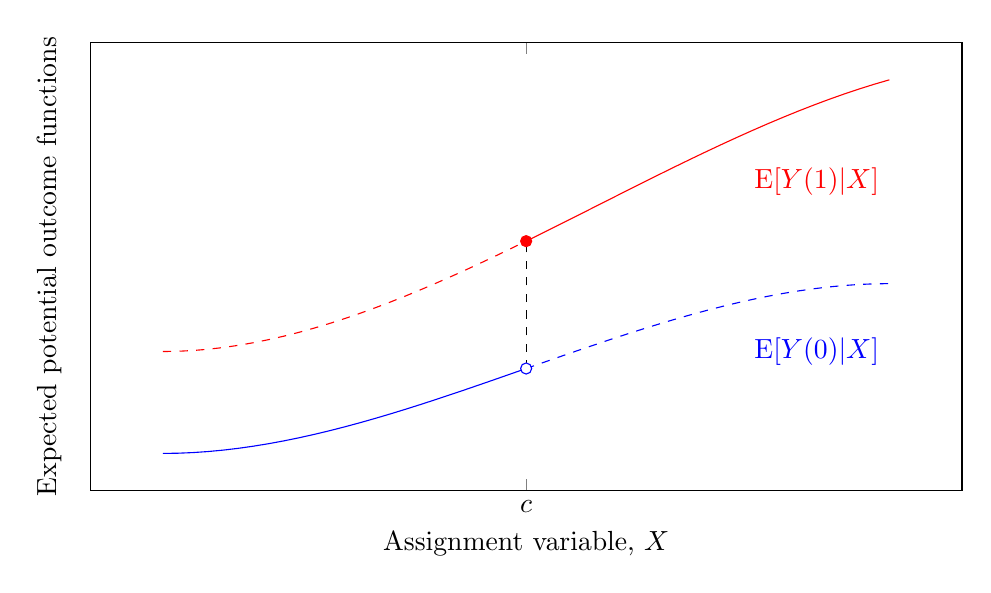
\begin{tikzpicture}
		\begin{axis}
			[
			width=1.5*240pt, height=207pt,
			xlabel={Assignment variable, $X$}, xtick={0.5}, xticklabels={$c$}, 
			ylabel={Expected potential outcome functions}, yticklabels={,,}, ytick style={draw=none} 
			]
			
			\addplot[blue, domain=0:0.5]
			expression{-0.5*x^3 + 0.75*x^2 + 0.3};
			
			\addplot[blue, dashed, domain=0.5:1]
			expression{-0.5*x^3 + 0.75*x^2 + 0.3};
			
			\addplot[red, domain=0.5:1]
			expression{-0.5*x^3 + 0.9*x^2 + 0.45};
			
			\addplot[red, dashed, domain=0:0.5]
			expression{-0.5*x^3 + 0.9*x^2 + 0.45};
			
			\addplot[blue, only marks, mark options={fill=white}]
			coordinates{(0.5, 0.425)};
			
			\addplot[red, only marks]
			coordinates{(0.5, 0.6125)};
			
			\draw[dashed] (0.5, 0.425) -- (0.5, 0.6125);
			
			\node[blue] at (axis cs:0.9, 0.45) {$\E[Y(0) | X]$};
			\node[red] at (axis cs:0.9, 0.7) {$\E[Y(1) | X]$};	
		\end{axis}
	\end{tikzpicture}
	\caption{Expected potential outcome function under control (in blue) and treatment (in red), respectively.
			 For units to the left of the cutoff $c$, we only observe control outcomes (according to the solid blue line) and no treatment outcomes (according to the dashed red line).
		 	 The opposite applies to units to the right of the cutoff.}
	\label{fig:regression_functions_SRDD}
\end{figure}
\noindent
Figure~\ref{fig:regression_functions_SRDD} illustrates this fundamental problem for the sharp design.
The figure shows two expected potential outcome functions, $\E[Y(0) | X=x]$ and $\E[Y(1) | X=x]$.
Both functions are plotted partly solid and partly dashed.
The reason is that in practice we can never observe realizations of the dashed function segments.
All units below the cutoff ($X_i < c$) are in the control group.
Thus, outcomes under treatment for this group are not observable (dashed red line).
All units above the cutoff ($X_i \geq c$) are treated.
Consequently, outcomes under control cannot be observed (dashed blue line).
Due to this lack of common support, the estimation of average (population) treatment effects, $\E[Y(1) - Y(0) | X = x]$, seems unfeasible.
In the next \hyperref[sec:identification]{section}, however, we state that under relatively mild conditions the average treatment effect (ATE) at the cutoff is identified in the sharp RD design.

\subsection{Fuzzy and other designs}  

In this thesis, we assume the basic RD setup, where all units comply with the treatment assignment (sharp design), there is one continuous assignment variable, and one cutoff.
In recent years, several extensions of the basic setup have been considered.
Especially, what is known as the fuzzy RD design.
In the fuzzy design there is still a discontinuity in the probability of receiving treatment at the cutoff, but not from zero to one.
The reason is imperfect compliance, i.e.\ some units assigned to control are treated, and/or some units supposed to be treated are not.
To give an example, in an early RD study, \textcite{Angrist_1999} investigate the effect of class size on scholastic achievement.
The authors exploit that primary schools in Israel are required to have no more than 40 pupils in a class.
Hence, at an enrollment-cutoff of 41, class size should drop sharply.
Some schools, however, still had classes with more than 40 pupils (e.g.\ due to scarcity of teachers), resulting in a fuzzy design.
An illustration of the conditional probability of being treated in a fuzzy design (with two-sided non-compliance) is depicted in Figure~\ref{fig:treatment_probability_FRDD}.
Such compliance issues hamper the treatment effect study, but many aspects from the sharp RD analysis carry over to the fuzzy case.
See, e.g., \textcite{Lee_2010}.

At this point, we just name a few other extensions.
The assignment variable can be discrete and have mass points \parencite{Kolesar_2018}.
A common example is age that is only available at an annual level.
RD designs can have multiple assignment variables \parencite{Papay_2011},
like two test scores (language and math).
A special case is the Geographic RD design, where treatment assignment changes at the border separating two areas.
Typically, latitude and longitude are then used for the analysis.
RD designs can also have multiple cutoffs but one assignment variable \parencite{Cattaneo_2016}.
For example, when regions choose a different cutoff to implement a federal program. 
% TeX file "identification"

% Master thesis 
% Sven Jacobs
% Winter 2022, M.Sc. Economics, Bonn University
% Supervisor: Prof. Dr. Dominik Liebl


\section{Identification} \label{sec:identification}

As described above, a fundamental problem is that we never observe treated and untreated units with the same value of the assignment variable.
Near the cutoff, though, we do observe treatment and control units, respectively, that exhibit a similar value of the assignment variable.
If in the absence of the treatment, the average potential outcomes would also be similar, we could compare these control and treatment units to learn about the average effect of the treatment near the cutoff.
\textcite{Hahn_2001} were the first to present a formal identification result motivated by this kind of continuity consideration. 

The key assumption to identify the sharp RD treatment effect
\begin{equation}
\tauSRD \equiv \E[Y(1) - Y(0) | X = c]
\end{equation}
is that the expected potential outcome functions are continuous at the cutoff.
That is, $\E[Y(0) | X = x]$ and $\E[Y(1) | X = x]$ are continuous at $x = c$.%
\footnote{Some researchers impose the stronger assumption that continuity holds over the full support (e.g.\ \cite{Imbens_2008}).}
Then, 
\begin{align}
	\tauSRD &= \lim_{x \downarrow c} \E[Y(1) | X = x] - \lim_{x \uparrow c} \E[Y(0) | X = x] \\
	&= \lim_{x \downarrow c} \E[Y | X = x] - \lim_{x \uparrow c} \E[Y | X = x] \,.
\end{align}
Therefore, the RD treatment effect can be estimated as the vertical distance between the two regression functions at the cutoff.
Under the continuity assumption, the average outcome of the units just below the cutoff constitutes a valid counterfactual for the just treated units.  
We also notice that for identification no additional covariates are required.
As we discuss later, however, covariates can be included to increase precision.

In Figure~\ref{fig:regression_functions_SRDD} both potential outcome functions are continuous in the assignment variable.
The treatment effect $\tau_{\SRD}$ is then identified as the vertical distance between the functions at the cutoff (dashed black line).

A peculiarity of the parameter $\tau_{\SRD}$ is its very local nature.
The sharp RD design can, in general, only recover the ATE at the cutoff.
That is, for units with an assignment value of $X_i = c$.
In general, the effect of the treatment is heterogeneous and varies with the assignment variable.
Without further assumptions, we cannot make any statement about the ATE for units away from the cutoff.
In the scenario of Figure~\ref{fig:regression_functions_SRDD}, the treatment effect $\tau_{\SRD}$ is indeed representative for the whole population,
due to the shape of the average potential outcome functions (approximately a homogeneous ATE).
In practice one would have to assume such shapes.
In the past years, different approaches have been suggested to increase the limited external validity of the RD treatment effect
(e.g.\ \textcite{Angrist_2015}, \textcite{Bertanha_2020}).

At the end of the section, we note that the continuity-based identification of RD effects following \textcite{Hahn_2001} is the standard.
Another framework for RD analysis assumes that the treatment is as-if randomly assigned near the cutoff.
In this randomization-based framework, the RD analysis is closely connected to the analysis of experiments (e.g.\ randomization inference).
The interested reader is referred to \textcite{Lee_2008}, and \textcite{Sekhon_2017}. 
% TeX file "estimation"

% Master thesis 
% Sven Jacobs
% Winter 2022, M.Sc. Economics, Bonn University
% Supervisor: Prof. Dr. Dominik Liebl


\section{Estimation} \label{sec:estimation}

Before turning to the main theoretical part, inference for the RD treatment effect, we discuss how to estimate the parameter $\tau_{\SRD}$,
which in the previous \hyperref[sec:identification]{section} was identified as the vertical distance between the regression functions at the cutoff.
The assignment variable $X$ is continuous.
Therefore, the estimation of $\E[Y(0) | X = c]$ and ${\E[Y(1) | X = c]}$ will rely on observations further away from the cutoff.
In the parametric approach, all observations are used to fit global polynomials (typically of higher order).
In the nonparametric approach, only observations near the cutoff are used to fit local polynomials (typically of lower order).
A challenge for either approach is that estimation occurs at a single point of interest, the cutoff, which is a boundary point.
After discussing the problems of the traditional parametric approach, we present the favorable local polynomial estimation.

\subsection{Parametric estimation: Global polynomials}

In the parametric estimation, for all $i = 1, \dots, n$ the model
\begin{equation}
	Y_i = \beta_0 + \alpha T_i + \beta_1(X_i-c) + \beta_2(X_i-c) T_i + \dots + \beta_{2p-1}(X_i-c)^p + \beta_{2p}(X_i-c)^p T_i + \varepsilon_i
\end{equation}
is postulated, where $p$ is the polynomial order.
Because the assignment variable is centered at the cutoff, $\hat{\alpha}$ constitutes the estimate of $\tauSRD$.
The interactions with the treatment indicator allow for a distinct influence of $X$ on the two groups.
In early applications the polynomials used to be of higher order (e.g.\ $p=4$ or $p=5$).
As usual, if the functional form is incorrectly specified, $\tauSRD$ is estimated with systematic bias.
But it also seems unappealing to include units far away from the cutoff for point estimation at the cutoff.
In a recent paper, \textcite{Gelman_2019} pointed out three major problems of higher-order polynomials in RD analyses and advise against their usage.
First, implicitly a high weight is given to units far from the cutoff.
Second, the estimator is sensitive to the degree of the polynomial.
And third, the confidence intervals have poor coverage.
For these reasons, RD estimation is now generally considered a nonparametric estimation problem.

\subsection{Nonparametric estimation: Local polynomials}

The most often applied estimation technique in RD analyses is local polynomial estimation.
The method approximates a function by locally fitting a polynomial, where the neighborhood is chosen by a bandwidth $h$.
Moreover, weights (based on a kernel function $K$) are assigned within the neighborhood, such that typically observations closer to the point of evaluation receive more weight.
Adapted for the sharp RD design, the estimation of $\tau_{\SRD}$ proceeds as follows.
We elaborate on each step below. \\

\noindent\fbox{%
	\parbox{\dimexpr\textwidth-2\fboxsep-2\fboxrule}{%
\begin{enumerate}
	\item Choose a kernel $K$ as the weighting scheme.
	\item Choose the order of the polynomial $p$.
	\item Choose the bandwidths $h_{\lowl}$ and $h_{\lowr}$.
	\item For control observations ($X_i < c$), fit a weighted least squares regression of order $p$ with weight $K \left( \frac{X_i-c}{h_{\lowl}} \right)$ for each observation:
		  \begin{equation}
		      \muhatlowl = \argmin_{\mulowl} \sum_{i: X_i<c} \{Y_i - \mulowl - \mulowlone(X_i - c) - \dots - \mulowlp(X_i - c)^p\}^2 K \left( \frac{X_i - c}{\hlowl} \right)
		  \end{equation}
	  	  The estimated intercept $\hat{\mu}_{\lowl}$ constitutes the estimate of $\E[Y(0) | X = c]$.
	\item For treatment observations ($X_i \geq c$), fit a weighted least squares regression of order $p$ with weight $K \left( \frac{X_i-c}{h_{\lowr}} \right)$ for each observation:
		  \begin{equation}
	          \muhatlowr = \argmin_{\mulowr} \sum_{i: X_i \geq c} \{Y_i - \mulowr - \mulowrone(X_i - c) - \dots - \mulowrp(X_i - c)^p\}^2 K \left( \frac{X_i - c}{\hlowr} \right)
		  \end{equation}
		  The estimated intercept $\hat{\mu}_{\lowr}$ constitutes the estimate of $\E[Y(1) | X = c]$.
	\item The estimated RD treatment effect is $\hat{\tau}_{\SRD} = \hat{\mu}_{\lowr} - \hat{\mu}_{\lowl}$. 
\end{enumerate}
	}%
}
\vspace{0.25cm}

The purpose of the kernel is to ensure that observations closer to the cutoff contribute more to the estimation at the cutoff.
The kernel most often applied in RD estimation is the triangular kernel, depicted in Figure~\ref{fig:kernels}.
The weight is maximized at the cutoff and declines linearly until an observation lies outside the interval $[c-h, c+h]$.
These observations receive zero weight.
It can be shown \parencite{Cheng_1997} that the triangular kernel is the (asymptotically) optimal kernel.
Nevertheless, in practice sometimes the uniform kernel assigning equal weights is used.
Another option is the Epanechnikov kernel with optimal properties for non-boundary estimation.\footnote{See Appendix~\hyperref[appendix:kernels]{1} for a comparison of the three kernels.}
The triangular kernel is recommended, albeit the particular choice is of minor importance.

As for the order of the local polynomial, an order of zero is discouraged for the RD design.
Estimation takes place at a boundary, i.e.\ only one-sided observations are available.
It is well known that the local constant estimator (so-called Nadaraya-Watson estimator) suffers from poor boundary behavior (e.g.\ \cite[Section~19.10]{Hansen_2022}).
By contrast, the local linear estimator ($p = 1$) was shown to be boundary-adaptive \parencite{Fan_1992}, leading to a boundary bias of lower order;
the same order as for estimation at interior points.
In general, a small $p \neq 0$ is preferable, as the trade-off between accuracy and variability should be governed by the bandwidth.
The default is local linear regression.
A data-driven polynomial order selection procedure was proposed by \textcite{Pei_2022}.

The bandwidth $h$ controls the size of the neighborhood around the cutoff, that is, how many observations are included for estimation.
The bandwidths $h_\lowl$ and $h_\lowr$, for estimation of $\E[Y(0) | X = c]$ and $\E[Y(1) | X = c]$, respectively, can differ in principle.
For example, a different bandwidth is reasonable when the data suggest a different degree of curvature.
In applications, often a common bandwidth $h = h_\lowl = h_\lowr$ is chosen.
In this thesis we restrict ourselves to the choice of a common bandwidth.
Bandwidth selection is a crucial and challenging step.
We address it in more detail below.

All estimation steps together are illustrated in Figure~\ref{fig:ll_estimation}.
In the example, the triangular kernel, $p = 1$, and a common bandwidth are applied.
According to steps (4) and (5), two weighted local linear regressions are fit separately (black lines).
The estimate $\tauhatSRD$ from step (6) is the difference between these two fitted regression lines at the cutoff $c$, which is close to the actual $\tauSRD$. 

\begin{figure}
	\centering
	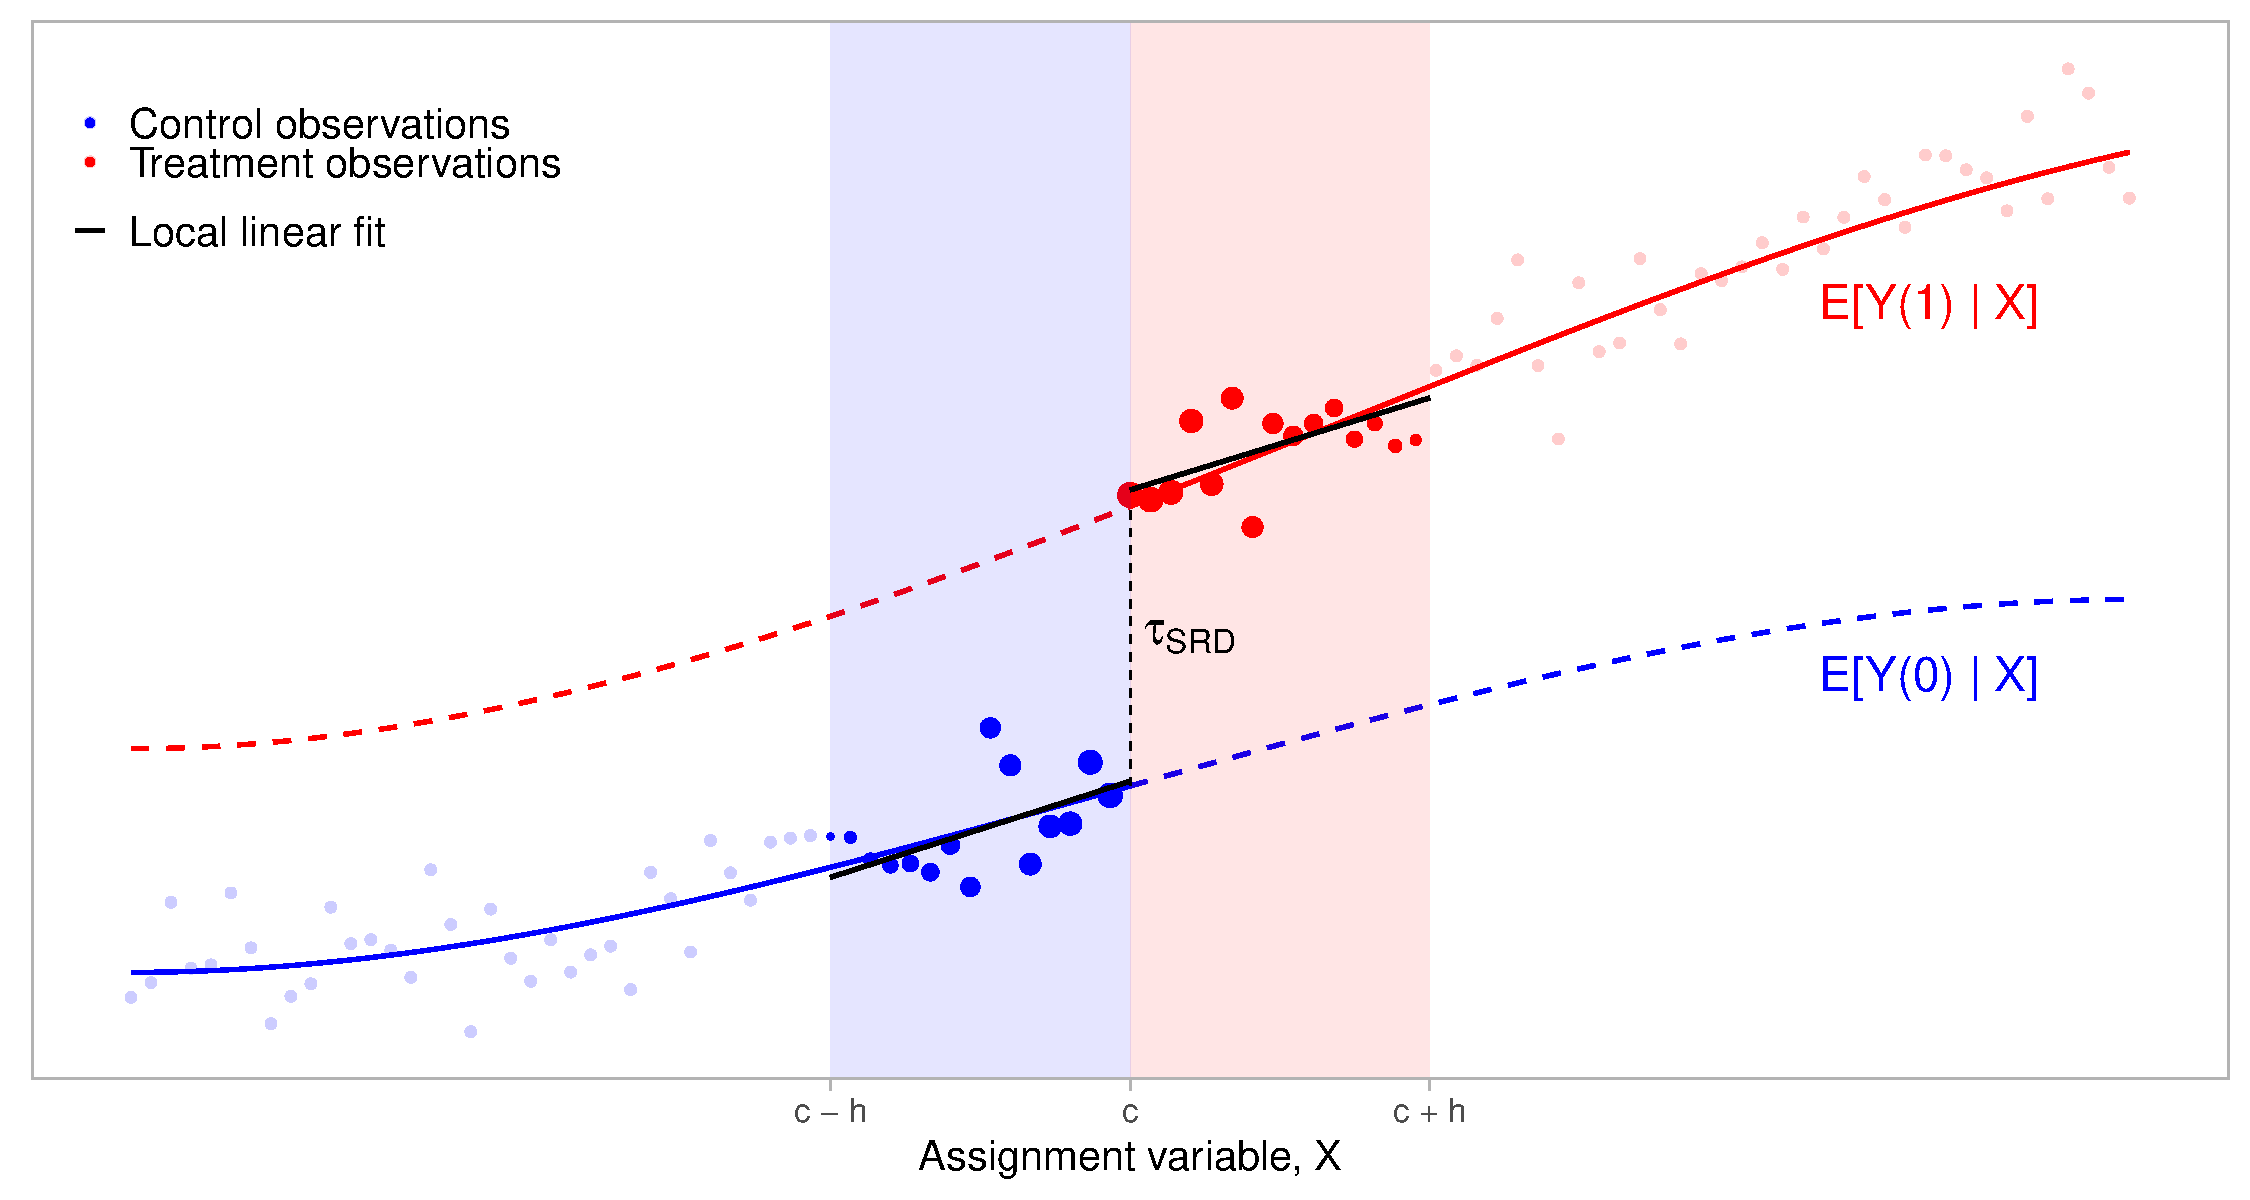
\includegraphics[width=\textwidth]{figure_03.pdf}
	\caption{Local linear estimation of the RD treatment effect $\tau_{\SRD}$.
			 Observed are random outcomes for the setting from Figure~\ref{fig:regression_functions_SRDD}.
		 	 The treatment effect is estimated by fitting locally a weighted linear regression, separately for control and treatment units.
	 	 	 The estimation windows, $[c - h, c]$ (control) and $[c, c + h]$ (treatment), are determined by the common bandwidth $h$.
 	 	 	 The weights, as given by the triangular kernel, are represented by the size of the dots in the shaded windows.}
	\label{fig:ll_estimation}
\end{figure}

\subsection{Bandwidth selection}

The bandwidth is referred to as the smoothing parameter.
Heuristically, a larger bandwidth leads to more (smoothing) bias, as the lower-order polynomial approximation of the unknown regression function near the cutoff gets worse.
At the same time, the variance of the estimator decreases, as more observations are used.
Analogously, a smaller bandwidth generally leads to less bias, but increased variance.
Therefore, the bandwidth selection involves a bias-variance trade-off.
In Figure~\ref{fig:ll_estimation} both functions are well approximated by a first-order polynomial in the respective neighborhood;
bias will be small.

An ad hoc way of choosing the bandwidth is by \enquote{eyeballing}.
However, RD estimation and inference results are sensitive to the bandwidth choice, requiring automatic, data-dependent procedures.
Two popular procedures are cross-validation (CV) and plug-in.
\textcite{Imbens_2008} proposed a version of CV specifically for the RD design, aimed at estimation at the boundary.
To obtain a bandwidth with higher accuracy near the cutoff,
it may be prudent to discard units far away from the cutoff before computing the CV criterion. 

The plug-in method for a common bandwidth consists of deriving an explicit formula for the bandwidth that minimizes an asymptotic approximation to the
mean squared error (MSE) of $\tauhatSRD$, and then to plug in estimators for the unknown quantities in this formula.
The asymptotic or leading (conditional) MSE of $\tauhatSRD$ is
\begin{equation}
	\AMSE(\tauhatSRD) = \ABias^2(\tauhatSRD) + \AVar(\tauhatSRD) \,.
\end{equation}
For the bias term it can be shown \parencite[Section~4.2.2]{Cattaneo_2020_book} that
\begin{equation} \label{eq:ABias}
	\ABias(\tauhatSRD) = h^{p+1} \mathcal{B} \,, 
\end{equation}
with
\begin{equation}
	\mathcal{B} = \mathcal{B}_\lowr - \mathcal{B}_\lowl \,,\quad \mathcal{B}_\lowl = \mu_\lowl^{(p+1)} B_\lowl \,,\quad \mathcal{B}_\lowr = \mu_\lowr^{(p+1)} B_\lowr \,,
\end{equation}
\begin{equation}
	\mu_\lowl^{(p+1)} \equiv \lim_{x \uparrow c} \frac{\diff^{p+1} \E[Y(0) | X = x]}{\diff x^{p+1}} \,,\quad  
	\mu_\lowr^{(p+1)} \equiv \lim_{x \downarrow c} \frac{\diff^{p+1} \E[Y(1) | X = x]}{\diff x^{p+1}} \,.
\end{equation}
The constants $B_\lowl$ and $B_\lowr$ depend on the chosen kernel $K$ and polynomial order $p$.
The derivatives are related to the approximation errors of the $p$th-order polynomial approximations.
For instance, in case of local linear regression the error is driven by the second derivative.
The error increases in the curvature of the regression function.
Notice that, if $\mu_\lowl^{(p+1)}$ equals $\mu_\lowr^{(p+1)}$, the bias term can be offset.\footnote{If $p$ is uneven (e.g.\ as in local linear estimation), then $B_\lowl = B_\lowr$. See \textcite[Lemma A.1]{Calonico_2014}.}
For the asymptotic (conditional) variance it can be shown that
\begin{equation} \label{eq:AVar}
	\AVar(\tauhatSRD) = \frac{1}{nh} \mathcal{V} \,, 
\end{equation}
with
\begin{equation}
	\mathcal{V} = \mathcal{V}_\lowl + \mathcal{V}_\lowr \,,\quad \mathcal{V}_\lowl = \frac{\sigma_\lowl^2}{f_X(c-)} V \,,\quad \mathcal{V}_\lowr = \frac{\sigma_\lowr^2}{f_X(c+)} V \,,
\end{equation}
\begin{equation}
	\sigma_\lowl^2 \equiv \lim_{x \uparrow c} \Var(Y(0) | X = x) \,,\quad  
	\sigma_\lowr^2 \equiv \lim_{x \downarrow c} \Var(Y(1) | X = x) \,,
\end{equation}
\begin{equation}
	f_X(c-) \equiv \lim_{x \uparrow c} f_X(x) \,,\quad  
	f_X(c+) \equiv \lim_{x \downarrow c} f_X(x) \,.
\end{equation}
The constant $V$ depends on the chosen kernel $K$ and polynomial order $p$.
The presence of the density of the assignment variable $f_X$ at the cutoff reflects that variance will be larger if fewer observations close to the cutoff are available.
Notice that due to local estimation the effective sample size is $nh$ and not $n$.

The bias-variance trade-off is formally expressed by the optimization problem
\begin{equation}
	\min_{h>0} \,\, \AMSE(\tauhatSRD) = h^{2(p+1)} \mathcal{B}^2 + \frac{1}{nh} \mathcal{V} \,.
\end{equation}
A smaller bandwidth leads to reduced bias, but larger variance, and vice versa.
The resulting (A)MSE-optimal bandwidth is
\begin{equation} \label{eq:hMSE}
	h_{\text{MSE}} = \left( \frac{\mathcal{V}}{2(p+1) \mathcal{B}^2} \right)^{1/(2p+3)} \cdot n^{-1/(2p+3)} \,.
\end{equation}
Thus, for the local linear estimator $h_{\text{MSE}} \sim n^{-1/5}$.
This bandwidth is not directly applicable, as several ingredients are unknown in practice and estimates need to be plugged in first.
The bias estimation is more involved.
Estimates of $\mu_\lowl^{(p+1)}$ and $\mu_\lowr^{(p+1)}$ are obtained by separate local polynomial regressions,
with polynomial order $q \geq p+1$ and preliminary bandwidth $b$.
This bandwidth often relies on a rule of thumb.
\textcite{Imbens_2012} were the first to implement a plug-in bandwidth selector according to \eqref{eq:hMSE}
by substituting consistent estimators, albeit for $p=1$ only.
The bandwidth selector of \textcite{Calonico_2014} instead applies for any $p$.
Besides, their selector improves on the estimation of the variance component $\mathcal{V}$ and how preliminary bandwidths are chosen.
Under standard assumptions, both estimators are consistent and optimal in the sense of \textcite{Li_1987}.
Also, in distinction to $h_{\text{MSE}}$, both incorporate a (positive) regularization term in the denominator
to adjust for potential low precision in estimating $\mu_\lowl^{(p+1)}$ and $\mu_\lowr^{(p+1)}$ \parencite[Section~4]{Imbens_2012}.
The motivation is that even when substantial curvature is present, due to low precision the estimated biases may be small,
resulting in a very large and poor-performing bandwidth.
% TeX file "inference"

% Master thesis 
% Sven Jacobs
% Winter 2022, M.Sc. Economics, Bonn University
% Supervisor: Prof. Dr. Dominik Liebl


\section{Inference} \label{sec:inference}

The estimator $\tauhatSRD$ is MSE-optimal when constructed with the MSE-optimal bandwidth (or two distinct MSE-optimal bandwidths).
In the next step, we want to conduct inference for $\tauSRD$, i.e.\ building confidence intervals and testing hypotheses.
Valid inference for the RD treatment effect, however, is non-trivial.
The challenge is the present bias associated with the nonparametric estimation.
Under suitable regularity conditions \parencite[Lemma~A.1]{Calonico_2014} it can be shown that as $n \rightarrow \infty$, $h \rightarrow 0$, $nh \rightarrow \infty$,
\begin{equation} \label{eq:asymp-normal}
	\frac{\tauhatSRD - \tauSRD}{\SE(\tauhatSRD)} - \frac{\Bias(\tauhatSRD)}{\SE(\tauhatSRD)} \overset{d}{\longrightarrow} \mathcal{N}(0, 1) \,,
\end{equation}
where the standard error $\SE(\tauhatSRD)$ estimates the standard deviation of $\tauhatSRD$.
The asymptotic distribution of the $t$-statistic is not centered at zero.    
Hence, if bias is not negligible, standard least squares inference (e.g.\ standard $t$-test) will be invalid.
A correct null hypothesis of no treatment effect would be over-rejected. 
Valid inference procedures have to be aware of the (unknown) bias and incorporate it in some way.
In the following, we present the three main bias-aware approaches.
Their performance in practice will be assessed and compared in a simulation study as well as an application to real data.

\subsection{Undersmoothing}

The first approach is called undersmoothing.
The idea is to employ conventional least squares inference by choosing a smaller (\enquote{undersmoothed}) bandwidth relative to the MSE-optimal one.
The theoretical argument is that shrinking the bandwidth at a faster rate, e.g.\ $h \sim n^{-\delta}$ with $\delta > 1/5$ for $p=1$, 
eliminates the bias in the approximate large-sample distribution.
Formally, the ratio of bias and standard error in \eqref{eq:asymp-normal} converges in probability to zero, $\Bias(\tauhatSRD) / \SE(\tauhatSRD) \overset{p}{\longrightarrow} 0$. 
An asymptotic $(1-\alpha)100\%$ confidence interval can then be constructed by 
\begin{equation}
	\text{CI}_{\text{US}} = \left[\, \tauhatSRD \pm |z_{\alpha/2}| \cdot \SE(\tauhatSRD) \,\right] \,,  
\end{equation}  
where $z_{\alpha}$ denotes the $\alpha$-quantile of the standard normal distribution and the subscript \enquote{US} refers to 
\enquote{Undersmoothing}.
For the standard error different suitable options are available.
The usual choice is a weighted nearest neighbor or Eicker-Huber-White estimator.
Alternatively an estimator based on $\AVar(\tauhatSRD)$ in \eqref{eq:AVar}.

There are some drawbacks with undersmoothing.
There exists no clear guidance on how much to undersmooth,
i.e.\ how much the bandwidth for constructing CI\textsubscript{US} should deviate from $h_{\text{MSE}}$.
In addition, a smaller bandwidth means that fewer observations are included and variance is increased.
Lastly, bias is still existent in finite samples.

\subsection{Robust bias-correction}

An alternative approach is to estimate the smoothing bias and to base inference on the bias-corrected estimate.
The $t$-statistic will be modified and we obtain bias-corrected confidence intervals, centered at the bias-corrected estimate.
Compared to undersmoothing, the MSE-optimal bandwidth (and hence the same data) can be used for estimation and inference.  
\textcite{Calonico_2014} proposed what they call a robust bias-correction, which accounts for the additional variability of the bias estimation.

In a first step, the leading bias $\ABias(\tauhatSRD)$ is estimated and removed from the point estimator $\tauhatSRD$.
From discussing bandwidth selection in the previous \hyperref[sec:estimation]{section}, we already know how an estimator (of $\mathcal{B}$ in \eqref{eq:ABias}) is constructed:
The unknown derivatives are estimated by preliminary local polynomial regressions, with a higher polynomial order $q \geq p+1$ and a separate bandwidth $b$.
The estimated bias is already available when the MSE-optimal bandwidth has been implemented for point estimation.

Standard bias-correction then would use the conventional $\SE(\tauhatSRD)$ for the confidence interval,
thereby ignoring the introduced variability from the additional bias-correction step.
This is known to translate into poor coverage in applications (e.g.\ \cite{Hall_1992}).
In their robust bias-correction, \textcite{Calonico_2014} account for the additional variability
by allowing the estimated bias to converge in distribution to a random variable and contribute to the distributional approximation of $\tauhatSRD$.
The new asymptotic variance is larger,
and the resulting standard error $\SE_{\text{RBC}}(\tauhatSRD)$ will be larger than $\SE(\tauhatSRD)$.
All together, an asymptotically valid ${(1-\alpha)100\%}$ confidence interval for $\tauSRD$ is
\begin{equation}
	\text{CI}_{\text{RBC}} = \left[\, \left(\tauhatSRD - \widehat{\ABias}(\tauhatSRD)\right) \pm |z_{\alpha/2}| \cdot \SE_{\text{RBC}}(\tauhatSRD) \,\right] \,,
\end{equation}
where the subscript \enquote{RBC} refers to \enquote{Robust Bias-Correction}.
The interval is not centered at the MSE-optimal estimate $\tauhatSRD$, instead it is centered at the bias-corrected estimate.

Building on this robust bias-correction procedure, \textcite{Calonico_2020} examine what would be an optimal bandwidth choice for inference
(as compared to the MSE-optimal bandwidth for point estimation).
The authors' objective is to minimize the coverage error (CE) of the robust bias-corrected confidence interval CI\textsubscript{RBC},
i.e.\ the discrepancy between the empirical coverage and the nominal level.
Their bandwidth $h_{\text{CE}}$ minimizes an asymptotic approximation to the coverage error of CI\textsubscript{RBC}.
Consequently, when constructed with the CE-optimal bandwidth, CI\textsubscript{RBC} will be both valid and CE-optimal in large samples.
Even though no closed-form solution for $h_{\text{CE}}$ exists, it declines at a faster rate than $h_{\text{MSE}}$ and is therefore undersmoothed:
$h_{\text{CE}} \sim n^{-1/(p+3)}$ compared to $h_{\text{MSE}} \sim n^{-1/(2p+3)}$.

\subsection{Inflated critical value} \label{sec:AK}

The third approach by \textcite{Armstrong_2020} takes the potential bias of $\tauhatSRD$ into account
by using a larger critical value compared to the conventional or undersmoothing confidence interval.
In the following we present the general concept, for (technical) details we refer to \citeauthor{Armstrong_2020} (\citeyear{Armstrong_2020}, \citeyear{Armstrong_2018}).

Let $\E_g[\tauhatSRD | X_1, \dots, X_n]$ denote the conditional expectation of $\tauhatSRD$ when the conditional expectation function $\E[Y | X=x]$ is $g$.
The authors assume that $g$ belongs to a certain class of functions $\mathcal{G}$ (described below),
and construct confidence intervals achieving asymptotically correct coverage uniformly over $\mathcal{G}$. 
The worst-case bias of $\tauhatSRD$ over the function class $\mathcal{G}$ is
\begin{equation}
	\overline{\Bias}(\tauhatSRD) \equiv \sup_{g \in \mathcal{G}} \, \bigl\lvert \E_g[\tauhatSRD | X_1, \dots, X_n] - \tauSRD \bigr\rvert \,.
\end{equation}
The second term in \eqref{eq:asymp-normal} is bounded in absolute value by $\overline{\Bias}(\tauhatSRD) / \SE(\tauhatSRD)$.
Then, asymptotically, the $(1-\alpha)$-quantile of the absolute value of the $t$-statistic is bounded by $\cv_{1-\alpha}(\overline{\Bias}(\tauhatSRD) / \SE(\tauhatSRD))$,
where $\cv_{1-\alpha}(r)$ corresponds to the $(1-\alpha)$-quantile of the $\lvert \mathcal{N}(r, 1) \rvert$ distribution. 
Thus, an asymptotically valid $(1-\alpha)100\%$ confidence interval is obtained as
\vspace{2ex}
\begin{equation}
	\text{CI}_{\text{AK}} = \left[\, \tauhatSRD \pm \cv_{1-\alpha}\left(\frac{\overline{\Bias}(\tauhatSRD)}{\SE(\tauhatSRD)}\right) \cdot \SE(\tauhatSRD) \,\right] \,,
\vspace{1ex}
\end{equation} 
where the subscript \enquote{AK} refers to \enquote{\citeauthor{Armstrong_2020}}.

\citeauthor{Armstrong_2020} consider two function classes.
For the description we focus on local linear estimation.
Let $g_\lowl(x) = g(x)\mathbf{1}(x<c)$ and $g_\lowr(x) = g(x)\mathbf{1}(x \geq c)$
denote the part of the conditional expectation function below and above the cutoff, respectively.
For the first class
\begin{equation}
	\mathcal{G}_{\text{SRD,Tay}}(M) = \left\{ g_\lowl + g_\lowr \,|\, g_\lowl, g_\lowr \in \mathcal{G}_{\text{Tay,2}}(M) \right\} \,,
\end{equation}
the function $g$ is assumed to lie in the second-order Taylor class $\mathcal{G}_{\text{Tay,2}}(M)$ on either side of the cutoff.
This Taylor class requires $g_\lowl$ and $g_\lowr$ to be twice differentiable in a neighborhood left and right to the cutoff, respectively,
with the second derivative bounded in absolute value by $M$ in that neighborhood.
The class does not impose smoothness away from the cutoff, which might be undesirable in empirical applications.
Therefore, for the alternative class
\begin{equation}
	\mathcal{G}_{\text{SRD,Höl}}(M) = \left\{ g_\lowl + g_\lowr \,|\, g_\lowl, g_\lowr \in \mathcal{G}_{\text{Höl,2}}(M) \right\} \,,
\end{equation}
the function $g$ is assumed to lie in the second-order Hölder class $\mathcal{G}_{\text{Höl,2}}(M)$ on either side of the cutoff.
That is, $g$ has to be twice differentiable on either side of the cutoff,
and $M$ bounds the magnitude of the second derivative globally.%
\footnote{For the definition of $\mathcal{G}_{\text{Tay,2}}(M)$ and $\mathcal{G}_{\text{Höl,2}}(M)$ see \textcite[16]{Armstrong_2020}.}

The smoothness constant $M$ needs to be specified.
However, to maintain validity uniformly over the whole function class,
without further restrictions $M$ has to be set manually and cannot be data-driven.
Therefore, the advice is to use problem-specific knowledge to decide what choice is reasonable a priori.
Otherwise, two methods can provide guidance.
First, it is possible to place a lower bound on $M$ from the data \parencite[Supplement]{Kolesar_2018}.
Second, under the restriction that the second derivative in a neighborhood of the cutoff
is bounded by the maximum second derivative of a $\tilde{p}$th-order global polynomial approximation,
the bound $M$ can be chosen by a global polynomial rule of thumb:
A global polynomial of order $\tilde{p}$ is fit on either side of the cutoff,
and $M$ estimated to be the largest second derivative \parencite[Supplement]{Armstrong_2020}.

The confidence interval CI\textsubscript{AK} can be either constructed with a bandwidth that is MSE-optimal or inference-optimal.
For the former case, \textcite{Armstrong_2020} derive the bandwidth minimizing the maximum MSE over the function class $\mathcal{G}$.
For the latter case, the bandwidth is optimized for length and coverage, and will be slightly oversmoothed.

\subsection{Including covariates}

We conclude the section with covariate-adjusted RD analysis.
Researchers may want to include additional covariates for two reasons.
First, to increase precision and obtaining shorter confidence intervals.
Second, to restore identification when control and treated units near the cutoff differ systematically,
rendering the assumption of continuity of the average potential outcomes implausible.
For the latter purpose, usually additional parametric assumptions are required if the estimation target remains $\tauSRD$.
In the following, we only consider covariate inclusion for efficiency gains.

Let $\bm{Z}_i(0)$ and $\bm{Z}_i(1)$ be two vectors of potential covariates,
where $\bm{Z}_i(0)$ contains the covariate values that would be observed under control, and $\bm{Z}_i(1)$ what would be observed under treatment.
The observed covariate vector for unit $i$ is then
\begin{equation}
	\bm{Z}_i = \begin{cases} 
		\bm{Z}_i(0) & , X_i < c \\
		\bm{Z}_i(1) & , X_i \geq c
	\end{cases} \,.
\end{equation}
A natural approach is to directly include the covariates in the local polynomial regression.
\textcite{Calonico_2019} recommend to do this linearly, additive-separably and without interacting the covariates with the treatment.
That is, adding $\bm{Z}_i$ to a fully interacted weighted local regression
(the latter is algebraically equivalent to the two-step estimation from above).
Let $\tautildeSRD$ denote the covariate-adjusted estimator.
The authors show that, when the covariates are included this way,
under weak regularity conditions a zero RD treatment effect on the covariates (i.e.\ $\E[\bm{Z}_i(1)-\bm{Z}_i(0) | X_i=c] = 0$)
is sufficient for $\tautildeSRD$ to consistently estimate $\tauSRD$.
The condition should hold, for example, for covariates determined prior to the treatment assignment.

Notice that including covariates results in general in a different bandwidth, as the optimal bandwidth formulas depend on the covariates.
% TeX file "validation"

% Master thesis 
% Sven Jacobs
% Winter 2022, M.Sc. Economics, Bonn University
% Supervisor: Prof. Dr. Dominik Liebl


\section{Validation} \label{sec:validation}

An important part of any RD analysis is to provide evidence for its validity.
Evidence that the RD design can be used to learn about the local effect of the treatment on the outcome of interest.
Even though the continuity assumption on the expected potential outcome functions cannot be tested itself,
we present different checks to offer indirect evidence.
It should also be emphasized that the graphical illustration of the RD design is a powerful first step.
A plot of the outcome against the assignment variable can reveal the presence or absence of a jump at the cutoff.
In addition, one gets an impression of the shape of the underlying functions.
For the sake of clarity, often local means after binning instead of all observations are displayed.
To indicate the overall structure of the data, global polynomial fits (separately for control and treatment) are added.
Graphical RD presentation and optimal bin selection is discussed by \textcite{Calonico_2015a}.

\subsection{Manipulation of the assignment variable}

When the treatment is beneficial, units being placed into control have an incentive to manipulate their value of the assignment variable.
Successful manipulation can result in units barely receiving treatment being systematically different from units barely missing treatment,
apart from the treatment status.
If these differences affect the outcome, the units close to the cutoff cannot be compared to each other.
Continuity of the average potential outcomes would be violated, and the RD design would be invalid.
A prominent example is the award of a scholarship when a pupil scores above a grade threshold in a test.
A certain type of parent (e.g.\ highly ambitious) of just-failing children might try to somehow get the score improved.
Assume the question is what effect the scholarship has on later academic achievement.
If these parents are successful, an RD design would likely be invalid.
The reason is that after manipulation the average potential academic achievement of pupils just receiving the scholarship is likely to be higher,
independently from the scholarship.
Besides formal testing, administrative knowledge about the treatment-assigning process is helpful to learn about potential manipulation.
In the scholarship example, for instance, information about the test design, grading process, grade threshold, how parents might appeal.
In some cases, based on this knowledge manipulation can credibly be ruled out.

When the assignment variable cannot be precisely manipulated, we expect a continuous distribution.
A systematic difference in the number of units near the cutoff would question the RD validity.
For example, when there are unexpectedly many pupils just above the grade threshold.
A carefully created histogram can reveal such a jump in the density.
A more formal way is a density-continuity-test, testing whether the density of the assignment variable is continuous at the cutoff 
(the null hypothesis).
Failing to reject provides evidence against manipulation.
Any such test proceeds by estimating the density near the cutoff, separately below and above the cutoff. 
\textcite{McCrary_2008} was the first to propose a test, \textcite{Cattaneo_2020} developed a superior implementation.
To illustrate, Figure~\ref{fig:McCrary} in the appendix shows two densities, one with and one without manipulation.

Another approach to detect manipulation is to check whether the units near the cutoff are similar with respect to covariates
that could not have been affected by the treatment (e.g.\ predetermined covariates).
For example, whether parents' education of both pupil types (score slightly below and slightly above, respectively) is similar.
A systematic difference would point to manipulative behavior.
A formal analysis consists in an RD analysis, replacing the outcome $Y$ with a covariate.   
For each covariate, a separate analysis (i.e.\ bandwidth selection, treatment effect estimation, bias-aware inference) is conducted.
We should not find jumps that are distinguishable from zero.

\subsection{Placebo cutoffs}

The key identification assumption in the sharp RD design, continuity of the average potential outcome functions at the cutoff, is inherently untestable.
What can be tested instead, is whether the respective function, $\E[Y(0) | X=x]$ for $x<c$ and $\E[Y(1) | X=x]$ for $x \geq c$,
is continuous away from the cutoff.
To do so, we perform an RD analysis for placebo cutoffs, where the treatment status does not change.
For placebo cutoffs below the true cutoff, only control observations are used.
For placebo cutoffs above, only treated observations.
\textcite{Imbens_2008} suggest to choose the two median values.  
If we find jumps away from the cutoff, that cannot be explained plausibly,
this would doubt the interpretation of a jump at the real cutoff as the treatment effect.

\subsection{Bandwidth sensitivity and donut holes}

Finally, it is always advisable to check how sensitive the results are to the bandwidth choice.
It is reassuring if the findings are stable for different neighborhoods.
A plot of the estimated treatment effect together with its robust confidence interval over a range of bandwidths is typically insightful.
We expect that, in line with the bias-variance trade-off,
for bandwidths larger than the MSE-optimal one the confidence intervals will get shorter but displaced.

Another sensitivity check is to exclude some of the closest observations to the cutoff from the RD analysis,
known as the donut-hole-approach \parencite{Barreca_2011}.
At first sight, it seems illogical to exclude the observations that are usually the most informative.
The motivation is that if manipulation has taken place, likely the units closest to the cutoff are involved.   
In practice, estimation and inference results for different sizes of the donut hole should be compared.
% TeX file "application"

% Master thesis 
% Sven Jacobs
% Winter 2022, M.Sc. Economics, Bonn University
% Supervisor: Prof. Dr. Dominik Liebl


\section{Application} \label{sec:application}

To illustrate all the discussed steps in a bias-aware sharp RD analysis (identification, estimation, inference, validation),
we present an extensive application before the simulation study,
which then investigates inferential performance exclusively.
For the implementation of the application and simulation,
we particularly make use of the two \textsf{R} packages \texttt{rdrobust} by \citeauthor{Calonico_2019} and \texttt{RDHonest} by \citeauthor{Armstrong_2020}.
All materials (data, code, etc.) to replicate the results are available on GitHub:
\url{https://github.com/svjaco/master_thesis}

Our application is based on a prominent paper by \citeauthor{Ludwig_2007} (\citeyear{Ludwig_2007}, \citetitle{Ludwig_2007}).
In 1965 the U.S. launched the federal poverty alleviation program \enquote{Head Start}, targeted at poor children.
To receive funding, counties had to apply to a competitive selection process.
However, the federal government provided assistance to the 300 poorest counties to develop funding proposals.
\textcite[e.g.\ Figure I and II]{Ludwig_2007} document that this grant-writing assistance substantially increased Head Start participation and funding.
For example, 80 percent of the 300 treated counties received funding.
In their main analysis, \citeauthor{Ludwig_2007} used a sharp RD design to determine the local effect of grant-writing assistance
on child mortality due to causes the program's goal was to reduce.%
\footnote{Alternatively, we can think about the effect as an intent-to-treat effect of Head Start funding.} 
For estimation local linear regression is applied, but the bandwidth is chosen ad hoc, and their inference procedure ignores any potential bias.
Therefore, we review the original analysis and conduct validation checks, optimal bandwidth selection and bias-aware inference,
which have been developed after the paper's publication.

Table~\ref{tab:overview} provides a summary.
\begin{table}
	\centering
	\captionabove{Overview Head Start data set}
	\label{tab:overview}
	\resizebox{\textwidth}{!}{%
	\begin{tabular}{l l l}  
		\toprule 
		Assignment variable $(X)$ & County poverty rate in 1960        & Min:\,15.21 | Mean:\,36.73 | Max:\,81.57 \\
		Outcome $(Y)$             & Average mortality rate per 100000, & Min:\,0 | Mean:\,2.17 | Max:\,73.53 \\
		                          & Head Start related causes,         & \\
		                          & Ages 5--9, 1973--83                & \\		                          
		Cutoff $(c)$              & $X = 59.1984$                      & Poverty rate of 300th poorest county \\
		Treatment $(T)$           & Grant-writing assistance           & \\
		Additional covariates     & 14 (post: 4, prior: 10)            & See Table~\ref{tab:covariates} \\
		Number of observations    & 2781                               & Control: 2487, Treatment: 294 \\
		\bottomrule
	\end{tabular}}	
\end{table}
The assignment variable is the county poverty rate, obtained from the 1960 U.S. Census.
The outcome is the average mortality rate per 100000 for children of age 5--9, during 1973--83,
due to Head Start related causes (mainly anemia, meningitis and respiratory problems).
A county receives the treatment of grant-writing assistance when its poverty rate is above the cutoff 59.1984.
The raw data are plotted in Figure~\ref{fig:scatter}.
We have data on 2781 counties, with 294 of them above the poverty cutoff, receiving treatment.
We obtain more insights from the standard RD plot in Figure~\ref{fig:rdplot_Y}.
\begin{figure}
	\centering
	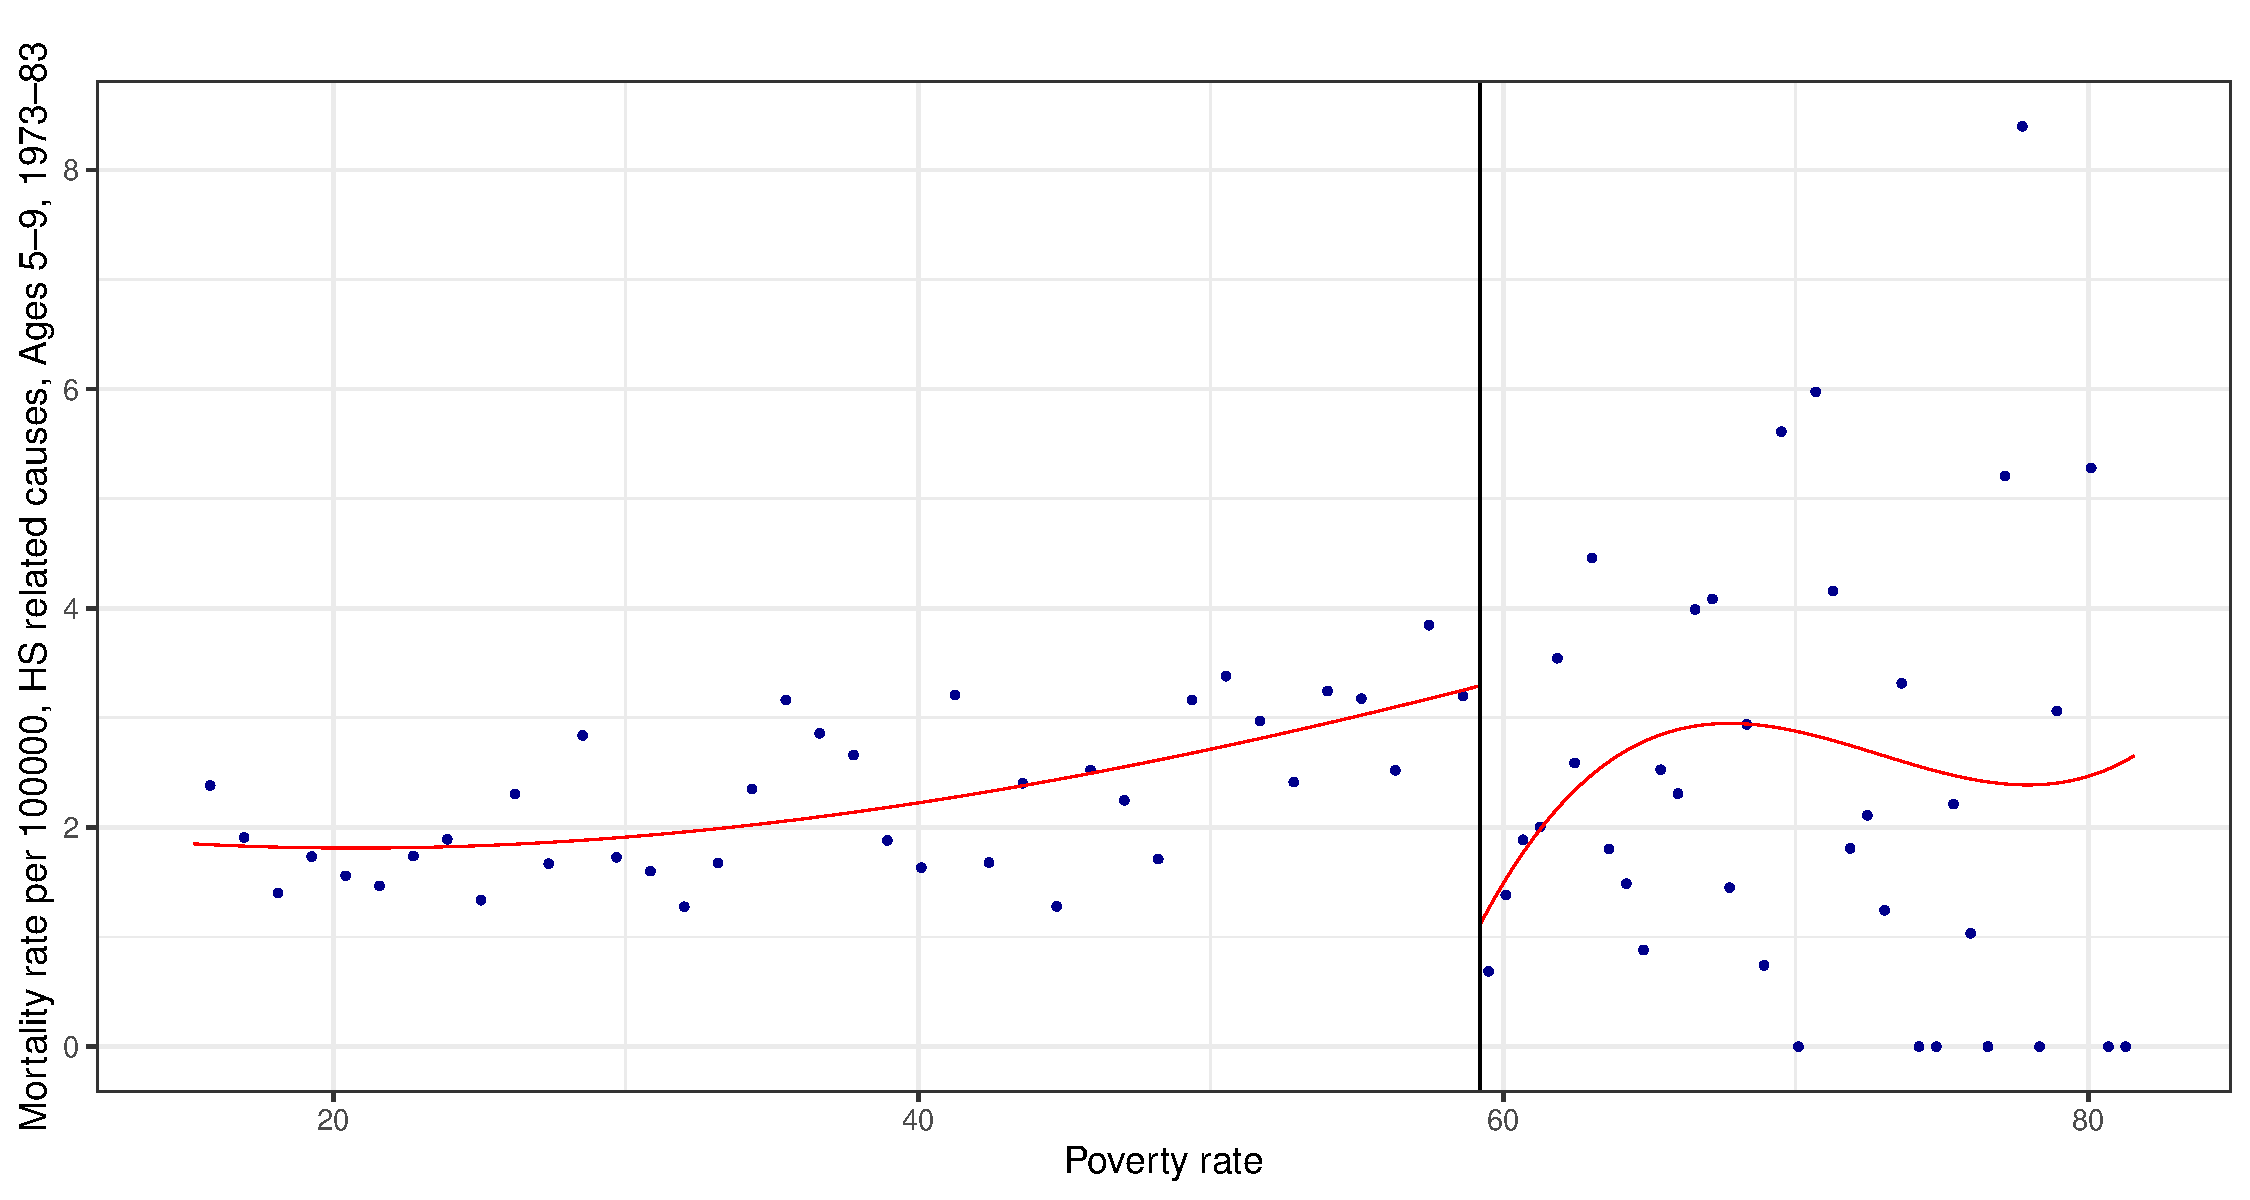
\includegraphics[width=\textwidth]{figure_04.pdf}
	\caption{Standard RD plot for the outcome of interest.
			 The dots depict the mean within each bin, where the bins are evenly spaced and their number is chosen to mimic the variance of the raw data (see \cite{Calonico_2015a}).
		 	 The solid red lines are third-order polynomial fits for control (left) and treated (right) counties separately.}
	\label{fig:rdplot_Y}
\end{figure}
The mortality rate increases nearly linearly in the poverty rate until the cutoff.
At the cutoff, the plot suggests a clearly visible downward discontinuity.
Afterwards, the mortality seems to rise nonlinearly.
Such a visualization provides valuable guidance, but can never replace a formal statistical treatment effect analysis
(remember the above mentioned problems of higher-order polynomial fitting).

The RD treatment effect $\tauSRD$ in the Head Start application is the ATE of receiving grant-writing assistance
on the Head Start (HS) related child mortality for a county with poverty rate in 1960 equal to 59.1984,
which reflects a very high poverty.
This effect can be identified with a sharp RD design if the continuity assumption holds.
That is, continuity (at the cutoff) of the expected potential mortality functions (with and without grant-writing assistance).
We have to be aware of two threats.
First, the cutoff might have been used in other federal social spending programs.
And second, the poverty rate might have been manipulated.
\citeauthor{Ludwig_2007} addressed the first concern and did not find any evidence for a discontinuity in other federal social spending at the Head Start cutoff.
Also, manipulation of the assignment variable can credibly been ruled out with the knowledge
that treatment was assigned in 1965 on the basis of official census information from 1960.
Nevertheless, we conduct the falsification tests from Section~\ref{sec:validation}.

The histogram of the poverty rate in Figure~\ref{fig:histogram} does not reveal any indication of sorting around the cutoff.
This is supported by a formal density-continuity-test, which clearly does not reject the null of continuity at the cutoff,
as illustrated in Figure~\ref{fig:rddensityplot}.
\begin{figure}
	\centering
	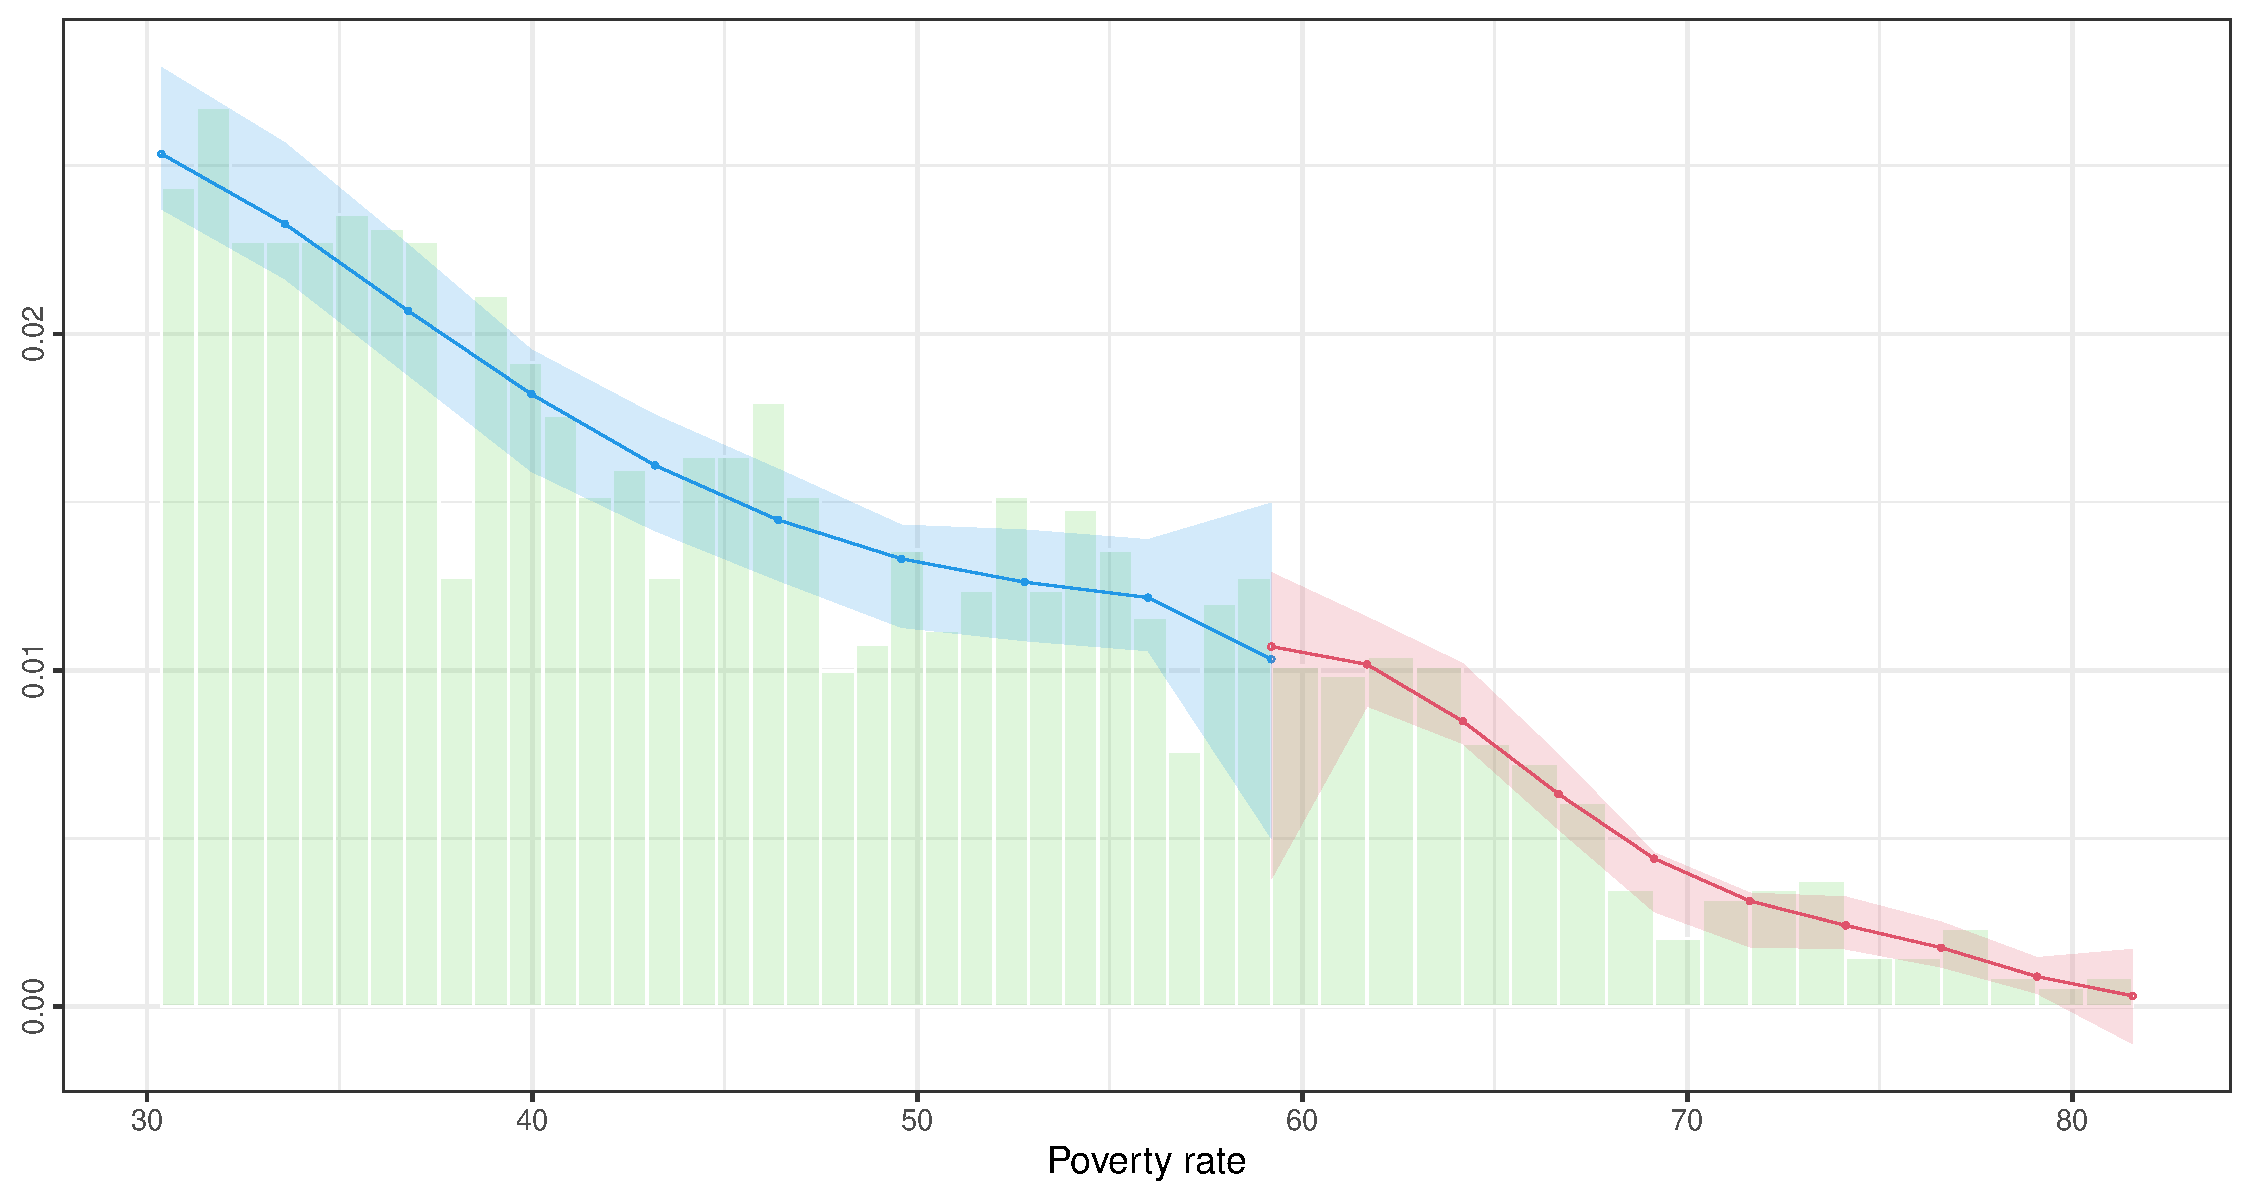
\includegraphics[width=\textwidth]{figure_05.pdf}
	\caption{Density-continuity-test for the poverty rate (assignment variable).
			 The density is estimated separately below (blue) and above (red) the cutoff,
		 	 using the local polynomial density estimator proposed by \textcite{Cattaneo_2020}.
	 	 	 The point estimates are non-centered, as the 95\% confidence intervals are robust bias-corrected.
 	 	 	 A histogram is added to the background.}
	\label{fig:rddensityplot}
\end{figure}
Next, we check whether statistically significant discontinuities can be found in variables where no treatment effect is expected.
For example, for other causes of death (mainly injuries) and the outcome of interest during the years 1959--64, before Head Start started.
For both variables we show the RD plot in Figure~\ref{fig:rdplots_cov}.
The plot for the pre-treatment HS related mortality does show a noticeable jump that requires further investigation.
Therefore, we perform a robust bias-corrected RD analysis and can debilitate the concern
(Figure~\ref{fig:llplot_Y_pre} combined with a robust $p$-value of 0.509 in Table~\ref{tab:covariates}).
The size of the jump in the RD plot is driven by the erratic behavior of the third-order polynomial at the cutoff.
Table~\ref{tab:covariates} reports the results of a separate RD analysis
(local linear estimation, triangular kernel, MSE-optimal bandwidth, RBC inference)
for each of the additional available covariates in the Head Start data set.
All 95\% robust confidence intervals contain zero.
For convenience the results are presented for the MSE-optimal instead of the CE-optimal bandwidth,
which might be a more suitable choice,
as we are mostly interested in inference here.
The conclusions, however, remain the same.
For completeness, we also report results from an RD analysis for placebo cutoffs (Table~\ref{tab:placebo_cutoffs})
and the donut-hole-approach (Table~\ref{tab:donut_holes}), as described at the end of Section~\ref{sec:validation}.
As a benchmark the results for $\tauhatSRD$ (i.e.\ effect at the true cutoff without excluded counties at the cutoff) are already included.
As expected, no significant effect at the artificial cutoffs occurs.
The donut-hole-analysis reveals that the results are somewhat sensitive to the degree of extrapolation at the cutoff.
Overall, the presented checks support the validity of the RD design. 

Let us now turn to the estimation of and inference for the effect of grant-writing assistance on the child mortality
(per 100000, ages 5--9, period 1973--83) due to HS related causes.
Our results are obtained for local linear estimation and the triangular kernel.
We consider the three bias-aware inference approaches from Section~\ref{sec:inference}:
undersmoothing, robust bias-correction, inflated critical value.
Standard errors are obtained via the nearest neighbor method.
The results are collected in Table~\ref{tab:HS_main} and visualized in Figure~\ref{fig:HS_main_plot}.
For the sake of comparison, the original findings from \textcite[Table~III]{Ludwig_2007} are reported as well.
Their bandwidths of $h^{\text{LM}}_1 = 9$ and $h^{\text{LM}}_2 = 18$ are ad hoc choices and
their inference procedure (bootstrapping the $t$-statistic) ignores potential bias.
Moreover, due to an error in the code, the applied kernel is the uniform kernel, and not (as stated) the triangular.
For the bandwidth of 9, \citeauthor{Ludwig_2007} report an estimate of $-1.895$, significant at the 5\% level.

\renewcommand{\arraystretch}{1.2}
\begin{table}[p]
	\centering
	\captionabove{Bias-aware analysis for the RD treatment effect in the Head Start application}
	\label{tab:HS_main}
	\resizebox{\textwidth}{!}{%
	\begin{tabular}{l l r c c c}  
		\toprule
		\multirow{2}[1]{*}{Approach} & \multicolumn{2}{c}{\multirow{2}[1]{*}{Bandwidth}} & \multirow{2}[1]{*}{RD estimate} & \multicolumn{2}{c}{Inference} \\
		\cmidrule(lr){5-6} 
		& & & & 95\% CI & $p$-value \\
		\midrule
		Undersmoothing                            & & & & & \\
		\quad -- By factor 2                      & $h^{\text{US}}_{1/2}$        & 3.457  & $-$3.428 & [$-$5.856, $-$1.001] & 0.006 \\
		\quad -- By factor 3                      & $h^{\text{US}}_{1/3}$        & 2.304  & $-$2.590 & [$-$5.488, 0.307]    & 0.080 \\
		Robust bias-correction                    & & & & & \\
		\quad -- MSE-optimal                      & $\hat{h}_{\text{MSE}}$       & 6.913  & $-$2.389 & [$-$5.426, $-$0.083] & 0.043 \\
		\quad -- CE-optimal                       & $\hat{h}_{\text{CE}}$        & 4.650  & $-$3.248 & [$-$6.092, $-$0.749] & 0.012 \\
		\quad -- MSE-optimal, incl. covariates    & $\tilde{h}_{\text{MSE}}$     & 7.115  & $-$2.445 & [$-$5.155, $-$0.339] & 0.025 \\
		\quad -- Ad hoc, \citeauthor{Ludwig_2007} & $h^{\text{LM}}_1$            & 9.000  & $-$2.182 & [$-$5.722, $-$0.350] & 0.027 \\
		\quad -- Ad hoc, \citeauthor{Ludwig_2007} & $h^{\text{LM}}_2$            & 18.000 & $-$1.681 & [$-$4.564, $-$0.101] & 0.040 \\
		\citeauthor{Armstrong_2020}               & & & & & \\
		\quad -- minimax MSE                      & $h^{\text{AK}}_{\text{MSE}}$ & 4.551  & $-$3.283 & [$-$6.039, $-$0.526] & 0.019 \\
		\quad -- Length-optimal                   & $h^{\text{AK}}_{\text{CIL}}$ & 4.670  & $-$3.239 & [$-$6.022, $-$0.456] & 0.022 \\
		\quad -- Ad hoc, \citeauthor{Ludwig_2007} & $h^{\text{LM}}_1$            & 9.000  & $-$2.182 & [$-$6.229, 1.866]    & 0.520 \\
		\quad -- Ad hoc, \citeauthor{Ludwig_2007} & $h^{\text{LM}}_2$            & 18.000 & $-$1.681 & [$-$11.700, 8.337]   & >0.9  \\
		\midrule
		\multicolumn{6}{l}{\citeauthor{Ludwig_2007} (bias ignored, uniform kernel)} \\
		\quad -- Ad hoc, \citeauthor{Ludwig_2007} & $h^{\text{LM}}_1$            & 9.000  & $-$1.895 &                      & 0.036 \\
		\quad -- Ad hoc, \citeauthor{Ludwig_2007} & $h^{\text{LM}}_2$            & 18.000 & $-$1.198 &                      & 0.081 \\                  
		\bottomrule \addlinespace[0.25ex]
		\multicolumn{6}{p{\dimexpr \textwidth+3\tabcolsep}}{\footnotesize \textit{Note}: Results are based on local linear estimation and the triangular kernel.
		The included additional covariates are all the variables from the Census 1960, as described in Table~\ref{tab:covariates}.
		For the approach by \citeauthor{Armstrong_2020}, the Hölder class and the global polynomial ROT $(M_{\text{ROT}}=0.299)$ are used.
		Due to an error in their code, the results from \textcite[Table~III]{Ludwig_2007} are obtained for the uniform kernel,
		and not (as reported) for the triangular.
		Their $p$-values are $t$-statistic-bootstrapped, ignoring potential bias.}
	\end{tabular}}	
\end{table}
\renewcommand{\arraystretch}{1.0}

\begin{figure}[p]
	\centering
	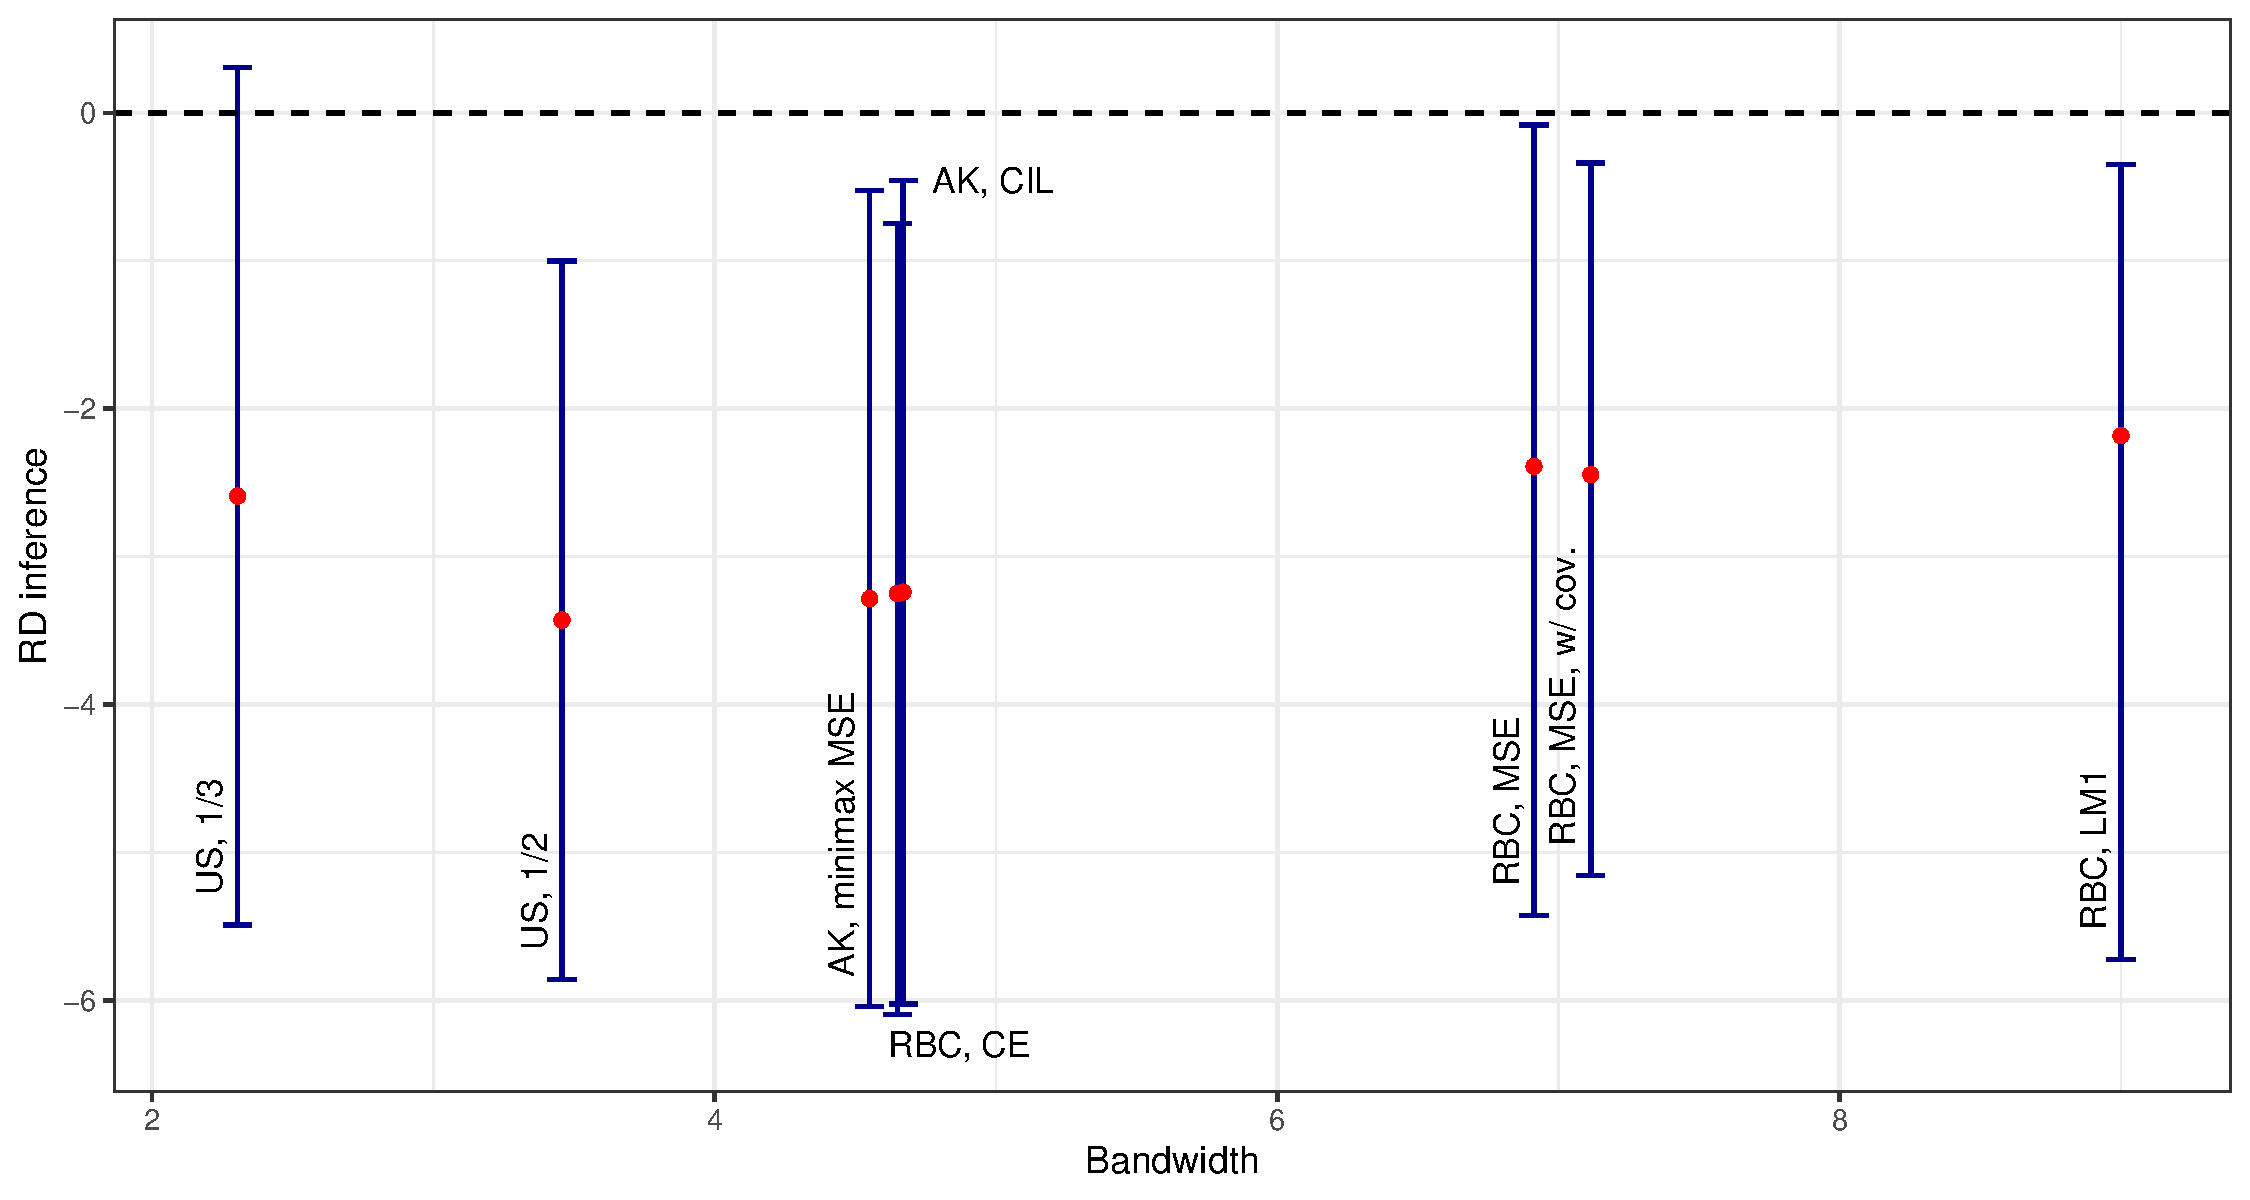
\includegraphics[width=\textwidth]{figure_06.pdf}
	\caption{Main results for the RD treatment effect in the Head Start application:
			 Point estimates and 95\% confidence intervals for the bias-aware inference approaches,
		 	 as presented in Table~\ref{tab:HS_main}.}
	\label{fig:HS_main_plot}
\end{figure}

We first compare with the RBC approach.
The estimated MSE-optimal bandwidth (using the plug-in selector of \cite{Calonico_2014}) is $\hat{h}_{\text{MSE}} = 6.913$,
leading to an estimated effect of $-2.389$ with robust $p$-value of 0.043.
Since the estimated untreated mortality at the cutoff for $\hat{h}_{\text{MSE}}$ is 3.585,
this is a large reduction of more than 60\%.
The MSE-optimal bandwidth suggests that the bandwidths of \citeauthor{Ludwig_2007} are too large (\enquote{oversmoothed}).
Including the nine predetermined variables from the U.S. Census 1960 (Table~\ref{tab:covariates})
showcases the potential gains from incorporating additional covariates.
The point estimate remains essentially the same, but the confidence interval is about 10\% tighter.
The CE-optimal bandwidth $\hat{h}_{\text{CE}} = 4.650$ is smaller and we obtain a larger (in magnitude) effect of $-3.248$.
To perform undersmoothing, we choose a bandwidth that is one half and one third of the MSE-optimal bandwidth, respectively.
Undersmoothing by 50\% yields the largest discontinuity out of all specifications ($-3.428$) and a relatively narrow confidence interval.
Estimating the bias for this undersmoothed bandwidth, however, indicates that bias is not negligible,
and the inference is too optimistic.
In contrast, for $h^{\text{US}}_{1/3}$ we get an estimate similar to the MSE-optimal one with a relatively wide confidence interval,
containing as the only one zero.
The third approach by \citeauthor{Armstrong_2020} requires the specification of the function class $\mathcal{G}$ and smoothness constant $M$ (Section~\ref{sec:AK}).
We choose the Hölder class (imposing smoothness away from the cutoff) and
the global polynomial rule of thumb to bound the second derivative of the conditional expectation function globally.
For these choices, the minimax bandwidth $h^{\text{AK}}_{\text{MSE}}$,
minimizing the maximum MSE of the local linear estimator over the specified class,
is 4.551 and thus 34\% smaller than $\hat{h}_{\text{MSE}}$.
The resulting RD estimate and confidence interval are close to the CE-optimal RBC results.
When the criterion is to optimize interval length while maintaining coverage, the bandwidth $h^{\text{AK}}_{\text{CIL}}$ is only slightly increased.

We conclude the following from the above presented.
Our results indicate that the bandwidths in the original paper are too large.
To theoretically justify these bandwidths within the approach of \citeauthor{Armstrong_2020},
the conditional expectation function has to be nearly linear (i.e.\ $M$ has to be substantially smaller).
This is not consistent with the data, when looking at the evolution of the average mortality rate in the treatment group in Figure~\ref{fig:rdplot_Y}.
Both, using the uniform kernel (estimate of $-1.895$ vs.\ $-2.182$ for the triangular kernel) and the oversmoothing
contribute to an understatement of the effect size.
Our bias-aware analysis yields larger confidence intervals (due to smaller bandwidths plus bias-awareness),
but at the same time larger treatment effects, leaving the original conclusion unchanged.
In summary, our analysis reaffirms the HS targeted mortality reducing effect of grant-writing assistance at the cutoff.

The application already indicates that how much to undersmooth is a delicate question,
and we might easily run into undercoverage if the bandwidth is still \enquote{too large}.
This is one of the points addressed in the upcoming simulation.  
% TeX file "simulation"

% Master thesis 
% Sven Jacobs
% Winter 2022, M.Sc. Economics, Bonn University
% Supervisor: Prof. Dr. Dominik Liebl


\section{Simulation}

To study the finite-sample performance of the asymptotically valid confidence intervals from Section~\ref{sec:inference},
we conduct a Monte Carlo experiment.
We compare empirical coverage and average interval length for three realistic conditional expectation functions.

\subsection{Setup}

The setup for the simulation study is the same as in \textcite{Calonico_2014},
which itself is based on the data generating process in \textcite{Imbens_2012}.
For each replication the data are generated as $n = 500$ i.i.d.\ draws, $i = 1, \dots, n$, from the model
\begin{align}
	Y_i &= \mu_{j}(X_i) + \varepsilon_i \,, \quad j = 1, 2, 3 \,, \\
	X_i &\sim 2 \Beta(2, 4) -1 \,, \\
	\varepsilon_i &\sim \mathcal{N}(0, 0.1295^2) \,,
\end{align}
where $\Beta(\alpha, \beta)$ denotes the beta distribution with shape parameters $\alpha$ and $\beta$,
and the index $j$ specifies the functional form of the conditional expectation function.
Three models are considered (Figure~\ref{fig:simulation_models}), with the following functional forms:
\begin{align}
	\mu_{1}(x) &=
	\begin{cases}
		0.48 + 1.27x + 7.18x^2 + 20.21x^3 + 21.54x^4 + 7.33x^5 & , x < 0 \\
		0.52 + 0.84x - 3.00x^2 + 7.99x^3 - 9.01x^4 + 3.56x^5   & , x \geq 0
	\end{cases} \,; \\
	\mu_{2}(x) &=
	\begin{cases}
		3.71 + 2.30x + 3.28x^2 + 1.45x^3 + 0.23x^4 + 0.03x^5 	 & , x < 0 \\
		0.26 + 18.49x - 54.81x^2 + 74.30x^3 - 45.02x^4 + 9.83x^5 & , x \geq 0 
	\end{cases} \,; \\ 
	\mu_{3}(x) &=
	\begin{cases}
		0.48 + 1.27x - 3.59x^2 + 14.147x^3 + 23.694x^4 + 10.995x^5 & , x < 0 \\
		0.52 + 0.84x - 0.30x^2 - 2.397x^3 - 0.901x^4 + 3.56x^5     & , x \geq 0 
	\end{cases} \,.
\end{align}
The first function $\mu_{1}(x)$ is obtained by fitting a fifth-order global polynomial 
with different coefficients for $X_i < 0$ and $X_i \geq 0$ to the data of
\citeauthor{Lee_2008} (\citeyear{Lee_2008}, \citetitle{Lee_2008}).
\citeauthor{Lee_2008} used an RD design to study the incumbency advantage in U.S. House elections. 
The second function $\mu_{2}(x)$ is obtained in the same way for the Head Start data \parencite{Ludwig_2007},
known from our application.
The assignment variable is rescaled to shift the cutoff to zero.
Notice that the population RD treatment effect according to $\mu_{2}$ is $-3.45$,
larger in magnitude than estimated in the application above.
Lastly, the specification $\mu_{3}(x)$ is obtained by altering some of the coefficients in Model~1,
in order to increase the overall curvature.
For convenience, the probability density function of $\Beta(2, 4)$ is plotted in Figure~\ref{fig:beta_pdf}.
On average, 18.75\% of the units will be in the treatment group (as $\Prob(Z \geq 0.5) = 0.1875$ for $Z \sim \Beta(2, 4)$).
In the Head Start application the share of treated counties was 10.57\%.   

\begin{figure}[p]
	\centering
	\begin{subfigure}{\textwidth}
		\centering
		\begin{tikzpicture}
			\begin{axis}
				[
				grid, grid style={white}, 
				samples=1000,
				ylabel={$\mu_{1}(X)$},
				]
				
				\addplot[black, domain=-1:0]
				{0.48 + 1.27*x + 7.18*x^2 + 20.21*x^3 + 21.54*x^4 + 7.33*x^5};
				\addplot[black, domain=0:1]
				{0.52 + 0.84*x - 3.00*x^2 + 7.99*x^3 - 9.01*x^4 + 3.56*x^5};
			\end{axis}
		\end{tikzpicture}
		\caption{Model 1 -- \textcite{Lee_2008}}
		\label{fig:model1}
	\end{subfigure}
	\\[3ex]
	\begin{subfigure}{\textwidth}
		\centering
		\begin{tikzpicture}
			\begin{axis}
				[
				grid, grid style={white}, 
				samples=1000,
				ylabel={$\mu_{2}(X)$},
				]
				
				\addplot[black, domain=-1:0]
				{3.71 + 2.30*x + 3.28*x^2 + 1.45*x^3 + 0.23*x^4 + 0.03*x^5};
				\addplot[black, domain=0:1]
				{0.26 + 18.49*x - 54.81*x^2 + 74.30*x^3 - 45.02*x^4 + 9.83*x^5};
			\end{axis}
		\end{tikzpicture}
		\caption{Model 2 -- \textcite{Ludwig_2007}}
		\label{fig:model2}
	\end{subfigure}
	\\[3ex]
	\begin{subfigure}{\textwidth}
		\centering
		\begin{tikzpicture}
			\begin{axis}
				[
				grid, grid style={white}, 
				samples=1000,
				ylabel={$\mu_{3}(X)$},
				]
				
				\addplot[black, domain=-1:0]
				{0.48 + 1.27*x - 3.59*x^2 + 14.147*x^3 + 23.694*x^4 + 10.995*x^5};
				\addplot[black, domain=0:1]
				{0.52 + 0.84*x - 0.30*x^2 - 2.397*x^3 - 0.901*x^4 + 3.56*x^5};
			\end{axis}
		\end{tikzpicture}
		\caption{Model 3}
		\label{fig:model3}
	\end{subfigure}
	\caption{Conditional expectation functions for the simulation study}
	\label{fig:simulation_models}
\end{figure}

\begin{figure}
	\centering
	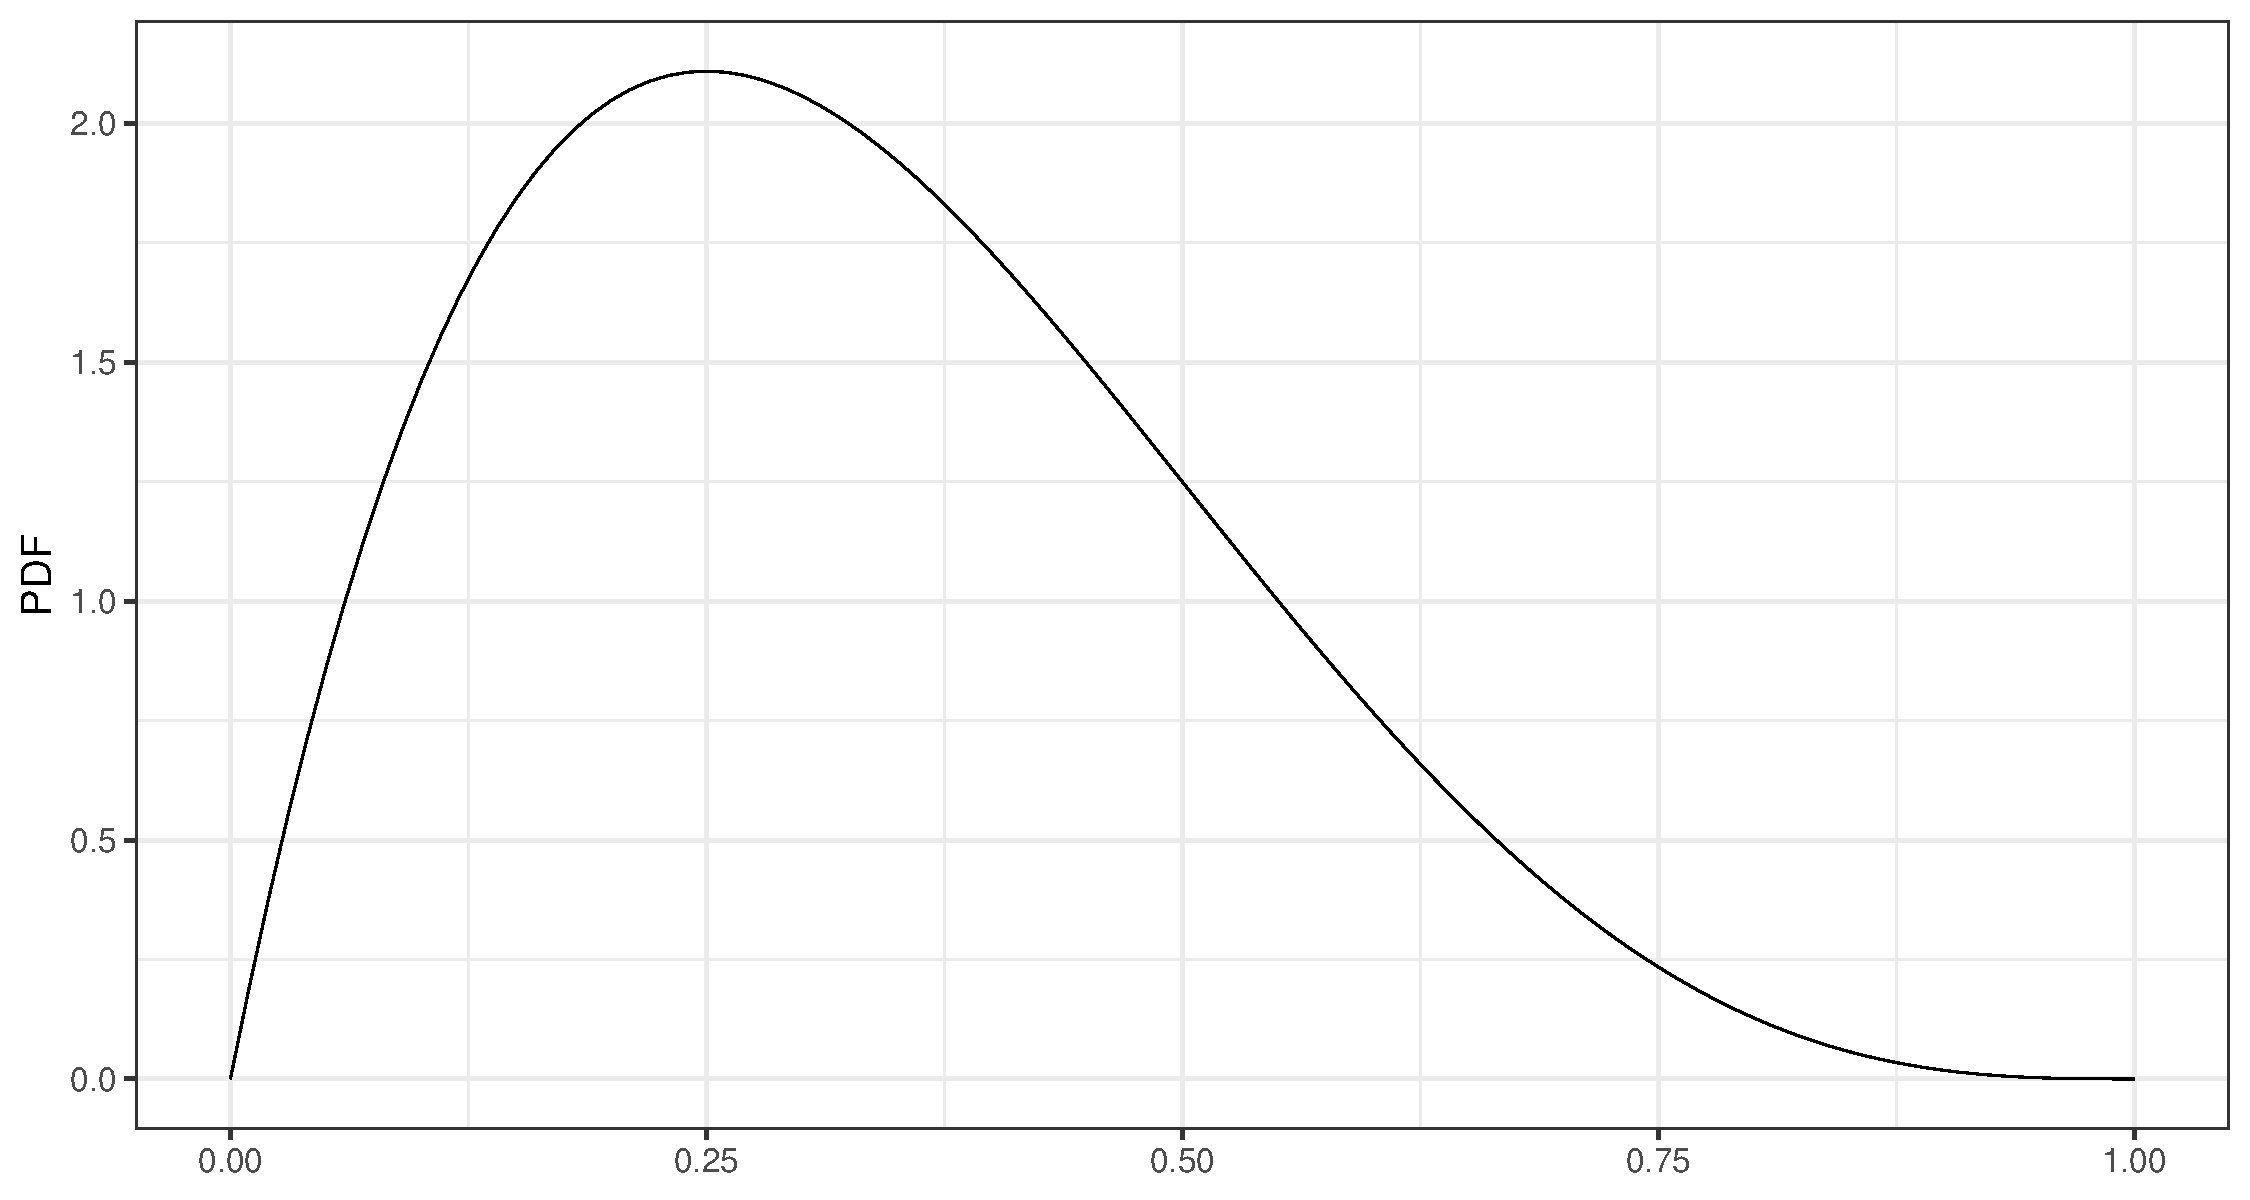
\includegraphics[width=\textwidth]{figure_08.pdf}
	\caption{Probability density function of the beta distribution $\Beta(\alpha, \beta)$
			 with shape parameters $\alpha = 2$ and $\beta = 4$}
	\label{fig:beta_pdf}
\end{figure}

For each model and bias-aware inference procedure we report the average bandwidth,
approximated bias and root MSE, empirical coverage and average interval length across 5000 replications.
We consider the following eight specifications:
Undersmoothing (ad hoc) by dividing the estimated MSE-optimal bandwidth by two and three,
robust bias-correction with bandwidths $\hat{h}_{\text{MSE}}$ and $\hat{h}_{\text{CE}}$,
and the approach by \textcite{Armstrong_2020} with the minimax MSE-optimal and length-optimal bandwidth
(respectively for the rule of thumb choice of the smoothness constant $M_{\text{ROT}}$ and the truth $\overbar{M}$).
In all cases, we conduct local linear estimation with the triangular kernel.
Standard errors are obtained by heteroskedasticity-robust nearest neighbor (with three as the minimum number of neighbors).
For reference, we also report the infeasible MSE-optimal bandwidth $h_{\text{MSE}}$,
which can be derived because of the known data generating process.
All confidence intervals are computed at the nominal 95\% coverage level. 

\subsection{Results and discussion}

The simulation results are collected in Table~\ref{tab:model1}, Table~\ref{tab:model2} and Table~\ref{tab:model3}.
We begin with Model~1 (\cite{Lee_2008}).
Due to the overall linear shape of $\mu_{1}$, the true MSE-optimal bandwidth $h_{\text{MSE}} = 0.166$ is relatively large.
The estimated version $\hat{h}_{\text{MSE}} = 0.196$ is larger,
and results for RBC in some undercoverage (91.70\%).
The CE-optimal bandwidth is substantially smaller and coverage is slightly improved.
For undersmoothing, bias can be reduced and coverage is similar to RBC with $\hat{h}_{\text{CE}}$,
but with wider confidence intervals (the cost of increased variance).
The results for the minimax MSE bandwidth for the correctly specified $\overbar{M}$ are very close to the CE-optimal RBC results in all aspects,
except for improved coverage of 95.38\%, almost exactly the nominal level.
Since the rule of thumb (ROT) calibrated choice is larger than $\overbar{M}$,
the corresponding bandwidth is smaller (as the maximal bias is larger).
The coverage is even better, at the expense of a slightly increased average interval length.
Results for the length-optimal bandwidth selector are essentially the same.
On balance, undersmoothing and RBC exhibit some degree of undercoverage,
with undersmoothing having on average the widest intervals.
In contrast, all specifications of the procedure by \citeauthor{Armstrong_2020} achieve accurate coverage.      

\renewcommand{\arraystretch}{1.2}
\begin{table}
	\centering
	\captionabove{Simulation results for Model 1 \parencite{Lee_2008} and nominal coverage of 95\%}
	\label{tab:model1}
	\resizebox{\textwidth}{!}{%
		\begin{tabular}{l c c c c c}  
			\toprule
			Approach & Bandwidth & Bias & RMSE & CI coverage [\%] & CI length \\
			\midrule
			Undersmoothing (ad hoc) & & & & & \\
			\quad -- By factor 2                       & 0.098 & 0.005 & 0.082 & 92.60 & 0.297 \\
			\quad -- By factor 3                       & 0.065 & 0.001 & 0.101 & 92.24 & 0.370 \\
			Robust bias-correction & & & & & \\
			\quad -- MSE-optimal                       & 0.196 & 0.019 & 0.064 & 91.70 & 0.246 \\
			\quad -- CE-optimal                        & 0.144 & 0.013 & 0.071 & 92.44 & 0.266 \\
			\citeauthor{Armstrong_2020} & & & & & \\
			\quad -- minimax MSE ($M_{\text{ROT}}$)    & 0.126 & 0.011 & 0.069 & 95.12 & 0.289 \\
			\quad -- minimax MSE ($\overbar{M}$)       & 0.146 & 0.014 & 0.063 & 95.38 & 0.266 \\
			\quad -- Length-optimal ($M_{\text{ROT}}$) & 0.130 & 0.011 & 0.068 & 95.50 & 0.289 \\   
		    \quad -- Length-optimal ($\overbar{M}$)    & 0.150 & 0.015 & 0.062 & 95.66 & 0.266 \\               
			\bottomrule \addlinespace[0.25ex]
			\multicolumn{6}{p{\dimexpr \textwidth+3\tabcolsep}}{\footnotesize \textit{Note}:
			The columns are average bandwidth, approximated bias and root MSE,
			empirical coverage and average interval length across the 5000 replications.
			The infeasible MSE-optimal bandwidth is $h_{\text{MSE}} = 0.166$.
			Results are based on local linear estimation and the triangular kernel.
			For the approach by \citeauthor{Armstrong_2020}, the Hölder class is used with
			$M$ as either the rule of thumb $M_{\text{ROT}}$ ($= 22.399$ on average) or the truth $\overbar{M}=14.36$.}
	\end{tabular}}	
\end{table}
\renewcommand{\arraystretch}{1.0}
\newpage
For the second model \parencite{Ludwig_2007} the infeasible MSE-optimal bandwidth is $h_{\text{MSE}} = 0.082$,
which is half the size compared to Model~1, as expected from looking at the plots in Figure~\ref{fig:simulation_models}.
Again, the estimate $\hat{h}_{\text{MSE}} = 0.1$ is too high ($\approx 20\%$) and the RBC method undercovers by two percentage points.
Unfortunately, undersmoothing led to some numerical instability during the simulations for Model~2.
The number of successful replications was too low to obtain reliable results.
The results for the four specifications of \citeauthor{Armstrong_2020} are similar to each other,
as the ROT estimate of $M$ is close to the true value.
The empirical coverage is by one to two percentage points above the nominal level.
Compared to RBC, we obtain longer confidence intervals,
because the relatively high curvature of $\mu_{2}$ is taken into account by accordingly increased critical values.

The results for Model~3 in Table~\ref{tab:model3} are similar to those for Model~1 in Table~\ref{tab:model1}.
The increased overall curvature translates into somewhat smaller bandwidths.
Now, empirical coverage for the ad hoc undersmoothing is slightly worse,
while it is slightly improved for RBC.
The higher degree of curvature means that the bound on the second derivative $M$ is enlarged,
widening on average the \citeauthor{Armstrong_2020} confidence intervals.
Interestingly, for Model~3 $M_{\text{ROT}}$ is considerably below $\overbar{M}$ and similar to $M_{\text{ROT}}$ for Model~1.
This bias of $M_{\text{ROT}}$, however, does not have a relevant impact on coverage (but tightens the intervals).       

\renewcommand{\arraystretch}{1.2}
\begin{table}[p]
	\centering
	\captionabove{Simulation results for Model 2 \parencite{Ludwig_2007} and nominal coverage of 95\%}
	\label{tab:model2}
	\resizebox{\textwidth}{!}{%
		\begin{tabular}{l c c c c c}  
			\toprule
			Approach & Bandwidth & Bias & RMSE & CI coverage [\%] & CI length \\
			\midrule
			Undersmoothing (ad hoc) & & & & & \\
			\quad -- By factor 2                       & 0.050 & NA & NA & NA & NA \\
			\quad -- By factor 3                       & 0.033 & NA & NA & NA & NA \\
			Robust bias-correction & & & & & \\
			\quad -- MSE-optimal                       & 0.100 & 0.048 & 0.098 & 92.98 & 0.345 \\
			\quad -- CE-optimal                        & 0.073 & 0.027 & 0.100 & 93.02 & 0.396 \\
			\citeauthor{Armstrong_2020} & & & & & \\
			\quad -- minimax MSE ($M_{\text{ROT}}$)    & 0.077 & 0.032 & 0.095 & 96.08 & 0.440 \\
			\quad -- minimax MSE ($\overbar{M}$)       & 0.075 & 0.031 & 0.095 & 96.62 & 0.447 \\
			\quad -- Length-optimal ($M_{\text{ROT}}$) & 0.080 & 0.035 & 0.095 & 96.16 & 0.442 \\   
			\quad -- Length-optimal ($\overbar{M}$)    & 0.078 & 0.033 & 0.094 & 96.80 & 0.448 \\               
			\bottomrule \addlinespace[0.25ex]
			\multicolumn{6}{p{\dimexpr \textwidth+3\tabcolsep}}{\footnotesize \textit{Note}:
			The columns are average bandwidth, approximated bias and root MSE,
			empirical coverage and average interval length across the 5000 replications.
			The infeasible MSE-optimal bandwidth is $h_{\text{MSE}} = 0.082$.
			Results are based on local linear estimation and the triangular kernel.
			For the approach by \citeauthor{Armstrong_2020}, the Hölder class is used with
			$M$ as either the rule of thumb $M_{\text{ROT}}$ ($= 103.418$ on average) or the truth $\overbar{M}=109.62$.
			Undersmoothing led to numerical instability, wherefore results are not available.}
	\end{tabular}}	
\end{table}
\renewcommand{\arraystretch}{1.0}

\renewcommand{\arraystretch}{1.2}
\begin{table}[p]
	\centering
	\captionabove{Simulation results for Model 3 and nominal coverage of 95\%}
	\label{tab:model3}
	\resizebox{\textwidth}{!}{%
		\begin{tabular}{l c c c c c}  
			\toprule
			Approach & Bandwidth & Bias & RMSE & CI coverage [\%] & CI length \\
			\midrule
			Undersmoothing (ad hoc) & & & & & \\
			\quad -- By factor 2                       & 0.087 & $-$0.004 & 0.086 & 91.90 & 0.314 \\
			\quad -- By factor 3                       & 0.058 & $-$0.003 & 0.107 & 91.76 & 0.393 \\
			Robust bias-correction & & & & & \\
			\quad -- MSE-optimal                       & 0.173 & $-$0.013 & 0.065 & 92.94 & 0.252 \\
			\quad -- CE-optimal                        & 0.127 & $-$0.006 & 0.072 & 92.96 & 0.275 \\
			\citeauthor{Armstrong_2020} & & & & & \\
			\quad -- minimax MSE ($M_{\text{ROT}}$)    & 0.119 & $-$0.007 & 0.071 & 95.94 & 0.301 \\
			\quad -- minimax MSE ($\overbar{M}$)       & 0.095 & $-$0.005 & 0.079 & 95.64 & 0.339 \\
			\quad -- Length-optimal ($M_{\text{ROT}}$) & 0.122 & $-$0.007 & 0.070 & 96.14 & 0.301 \\   
			\quad -- Length-optimal ($\overbar{M}$)    & 0.098 & $-$0.005 & 0.077 & 96.08 & 0.339 \\               
			\bottomrule \addlinespace[0.25ex]
			\multicolumn{6}{p{\dimexpr \textwidth+3\tabcolsep}}{\footnotesize \textit{Note}:
			The columns are average bandwidth, approximated bias and root MSE,
			empirical coverage and average interval length across the 5000 replications.
			The infeasible MSE-optimal bandwidth is $h_{\text{MSE}} = 0.260$.
			Results are based on local linear estimation and the triangular kernel.
			For the approach by \citeauthor{Armstrong_2020}, the Hölder class is used with
			$M$ as either the rule of thumb $M_{\text{ROT}}$ ($= 26.629$ on average) or the truth $\overbar{M}=45.406$.}
	\end{tabular}}	
\end{table}
\renewcommand{\arraystretch}{1.0}

We summarize the Monte Carlo study as follows.
Undersmoothing achieves a decent coverage, but overall offers the worst combination of coverage and average interval length.
Robust bias-correction undercovers the true treatment effect slightly (similar to undersmoothing),
but yields the shortest intervals.
The CE-optimal bandwidth choice offers some small refinements in empirical coverage relative to the MSE-optimal bandwidth selector.
The best coverage is obtained for the procedure of \citeauthor{Armstrong_2020}.
The global polynomial rule of thumb to choose the required smoothness constant $M$ works reasonably well.
Still, the necessity to specify this constant to bound the second derivative on both sides of the cutoff constitutes a drawback.
Each method, however, imposes (explicitly or implicitly) restrictions on the smoothness of the conditional expectation function.
Estimating the bias in RBC via local quadratic regression assumes that (in a neighborhood around the cutoff)
the regression functions are three times continuously differentiable.
The Monte Carlo experiment suggests to report in practice the confidence intervals of \citeauthor{Armstrong_2020},
$\text{CI}_{\text{AK}}(h^{\text{AK}}_{\text{MSE}}, M_{\text{ROT}})$ and $\text{CI}_{\text{AK}}(h^{\text{AK}}_{\text{CIL}}, M_{\text{ROT}})$,
together with the robust bias-corrected confidence intervals,  
$\text{CI}_{\text{RBC}}(\hat{h}_{\text{MSE}})$ and $\text{CI}_{\text{RBC}}(\hat{h}_{\text{CE}})$.
In doing so, we can likely complement a more accurate but wider interval with a tighter but less accurate interval.
The sensitivity of the confidence intervals to the choice of the bandwidth and smoothing constant can then be further examined.
% TeX file "conclusion"

% Master thesis 
% Sven Jacobs
% Winter 2022, M.Sc. Economics, Bonn University
% Supervisor: Prof. Dr. Dominik Liebl


\section{Conclusion} \label{sec:conclusion}

This thesis provided an overview and illustration of modern (sharp) RD analysis
that takes potential bias into account to obtain valid inference for
the nonparametrically estimated RD treatment effect.
We discussed identification, estimation, validation and
presented the three main bias-aware inference approaches:
undersmoothing, robust bias-correction \parencite{Calonico_2014}, and inflated critical values \parencite{Armstrong_2020}.
We reanalyzed an older prominent RD study by \textcite{Ludwig_2007},
particularly by conducting bias-aware inference,
which provided support for the original findings.
In a Monte Carlo study we assessed and compared the finite-sample performance of the asymptotically valid inference procedures.
Based on the insights from all the parts, we discourage the application of ad hoc undersmoothing,
especially as the main approach to achieve valid bias-aware inference.
Instead, we recommend to report results for the two other approaches with the corresponding optimal bandwidth choices,
and the rule of thumb $M_{\text{ROT}}$ if no problem-specific knowledge for the choice is available.
If necessary, further sensitivity checks for the confidence intervals can be conducted.

The Monte Carlo experiment can be extended in several directions.
To ensure that the results are not sensitive to the chosen data generating process,
we can alter the distribution of the assignment variable (e.g.\ to a uniform distribution),
and the distribution of the error (e.g.\ to a log-normal distribution).
Furthermore, we can consider heteroskedastic errors, a different error variance, and a different sample size.
A natural extension of this thesis is bias-aware inference in fuzzy regression discontinuity designs.

\clearpage

% TeX file "appendix"

% Master thesis 
% Sven Jacobs
% Winter 2022, M.Sc. Economics, Bonn University
% Supervisor: Prof. Dr. Dominik Liebl


\phantomsection 
\addcontentsline{toc}{section}{Appendix} 

\section*{Appendix}

\renewcommand{\thefigure}{A\arabic{figure}}
\setcounter{figure}{0}
\renewcommand{\thetable}{A\arabic{table}}
\setcounter{table}{0}

\subsection*{Appendix 1: Kernels} \label{appendix:kernels}

\renewcommand{\arraystretch}{1.4}	
\begin{table}[h]
	\centering
	\captionabove{Prominent kernel functions}
	\label{tab:kernels}
	\begin{tabular}{l l c}  
		\toprule
		Kernel & Function & Support \\
		\midrule
		Triangular   & $K_\text{T}(u) = 1 - |u|$       & $[-1, 1]$ \\
		Uniform      & $K_\text{U}(u) = 0.5$           & $[-1, 1]$ \\
		Epanechnikov & $K_\text{E}(u) = 0.75(1 - u^2)$ & $[-1, 1]$ \\
		\bottomrule
	\end{tabular}	
\end{table}
\renewcommand{\arraystretch}{1.0}

\begin{figure}[h]
	\centering
	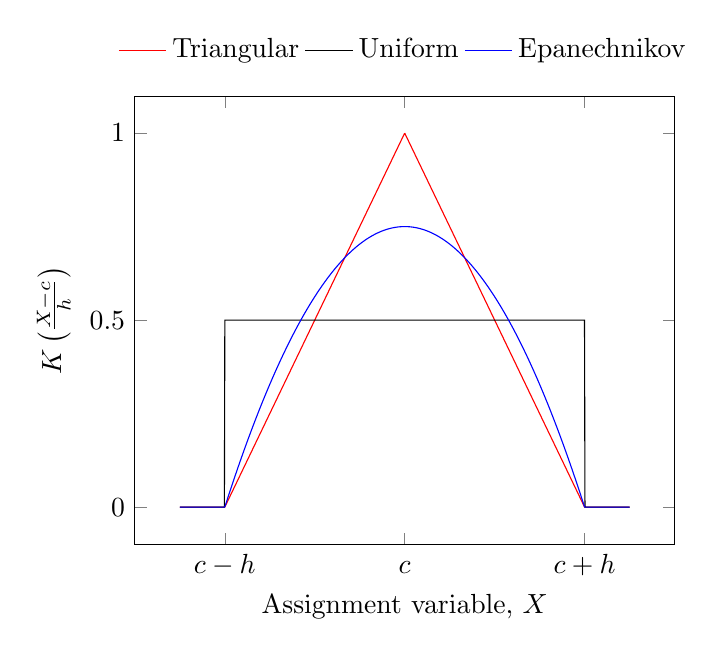
\begin{tikzpicture}
		\begin{axis}
			[
			grid, grid style={white}, 
			samples=1000, 
			domain=-1.25:1.25, 
			xlabel={Assignment variable, $X$}, xtick= {-1, 0, 1},
			xticklabels={$c-h$, \textcolor{white}{h}$c$\textcolor{white}{h}, $c+h$}, 
			ylabel=$K\left(\frac{X-c}{h}\right)$, ytick={0, 0.5, 1},
			legend entries={Triangular, Uniform, Epanechnikov},
			legend style={draw=none}, legend columns=3, legend style={at={(0.5, 1.05)}, anchor=south}
			]
			
			\addplot[red]
			expression {(1 - abs(x)) * (abs(x)<1)};
			
			\addplot[black]
			expression {1/2 * (abs(x)<1)};
			
			\addplot[blue]
			expression {3/4 * (1 - x^2) * (abs(x)<1)};
		\end{axis}
	\end{tikzpicture}
	\caption{Commonly used kernels as given in Table~\ref{tab:kernels}, applied to the RD design}
	\label{fig:kernels}
\end{figure}

\clearpage

\subsection*{Appendix 2: Manipulation of the assignment variable} \label{appendix:manipulation}

\begin{figure}[h]
	\centering
	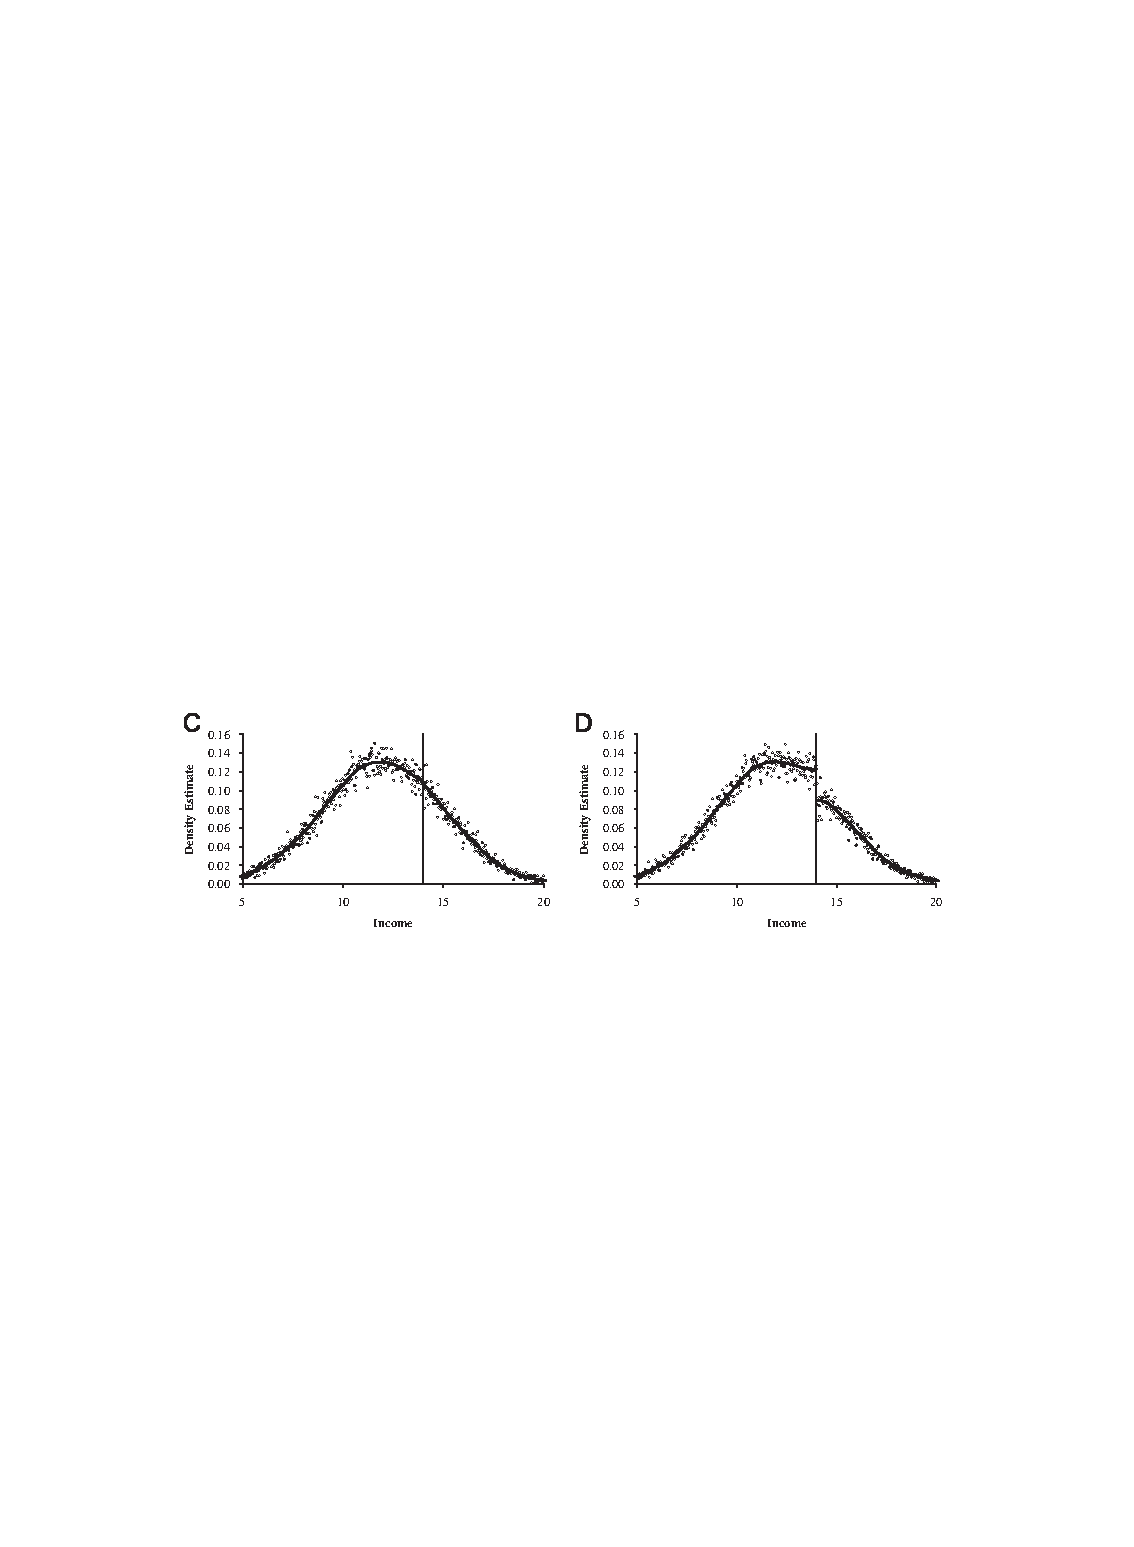
\includegraphics[width=\textwidth]{figure_A02.pdf}
	\caption{Hypothetical example of an income-tested job training program.
			 (C) density of income without manipulation; (D) density of income with manipulation.
		 	 From \textcite[Fig.~2]{McCrary_2008}.}
	\label{fig:McCrary}
\end{figure}

\clearpage

\subsection*{Appendix 3: Application} \label{appendix:application}
\vfill
\begin{figure}[h!]
	\centering
	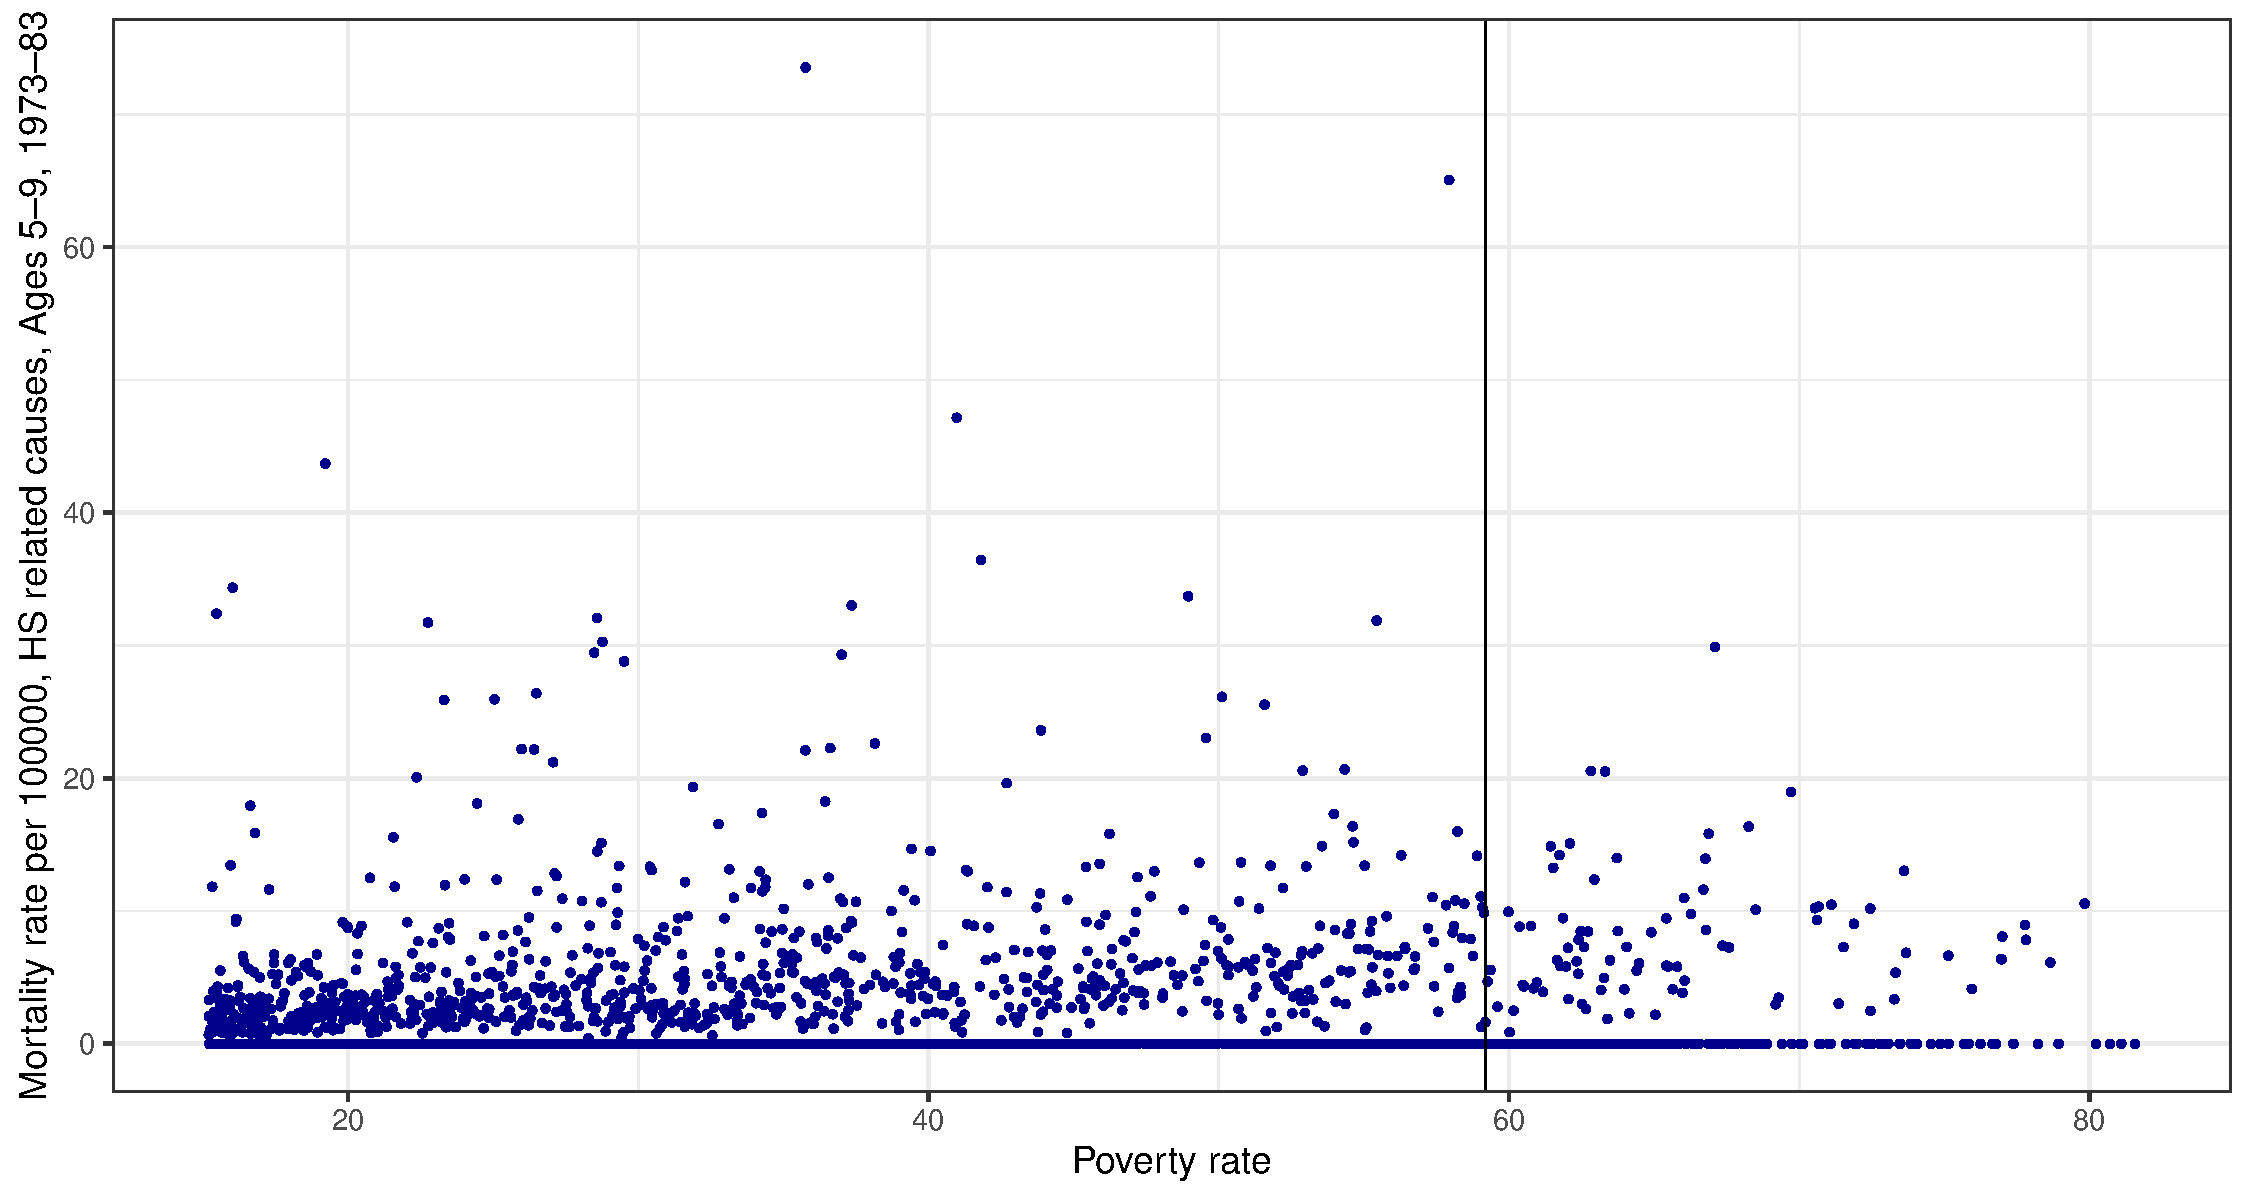
\includegraphics[width=\textwidth]{figure_A03.pdf}
	\caption{Scatter plot of the raw data underlying the Head Start RD analysis.
			 The cutoff of 59.1984 is indicated by the vertical line.}
	\label{fig:scatter}
\end{figure}
\vfill
\begin{figure}[h!]
	\centering
	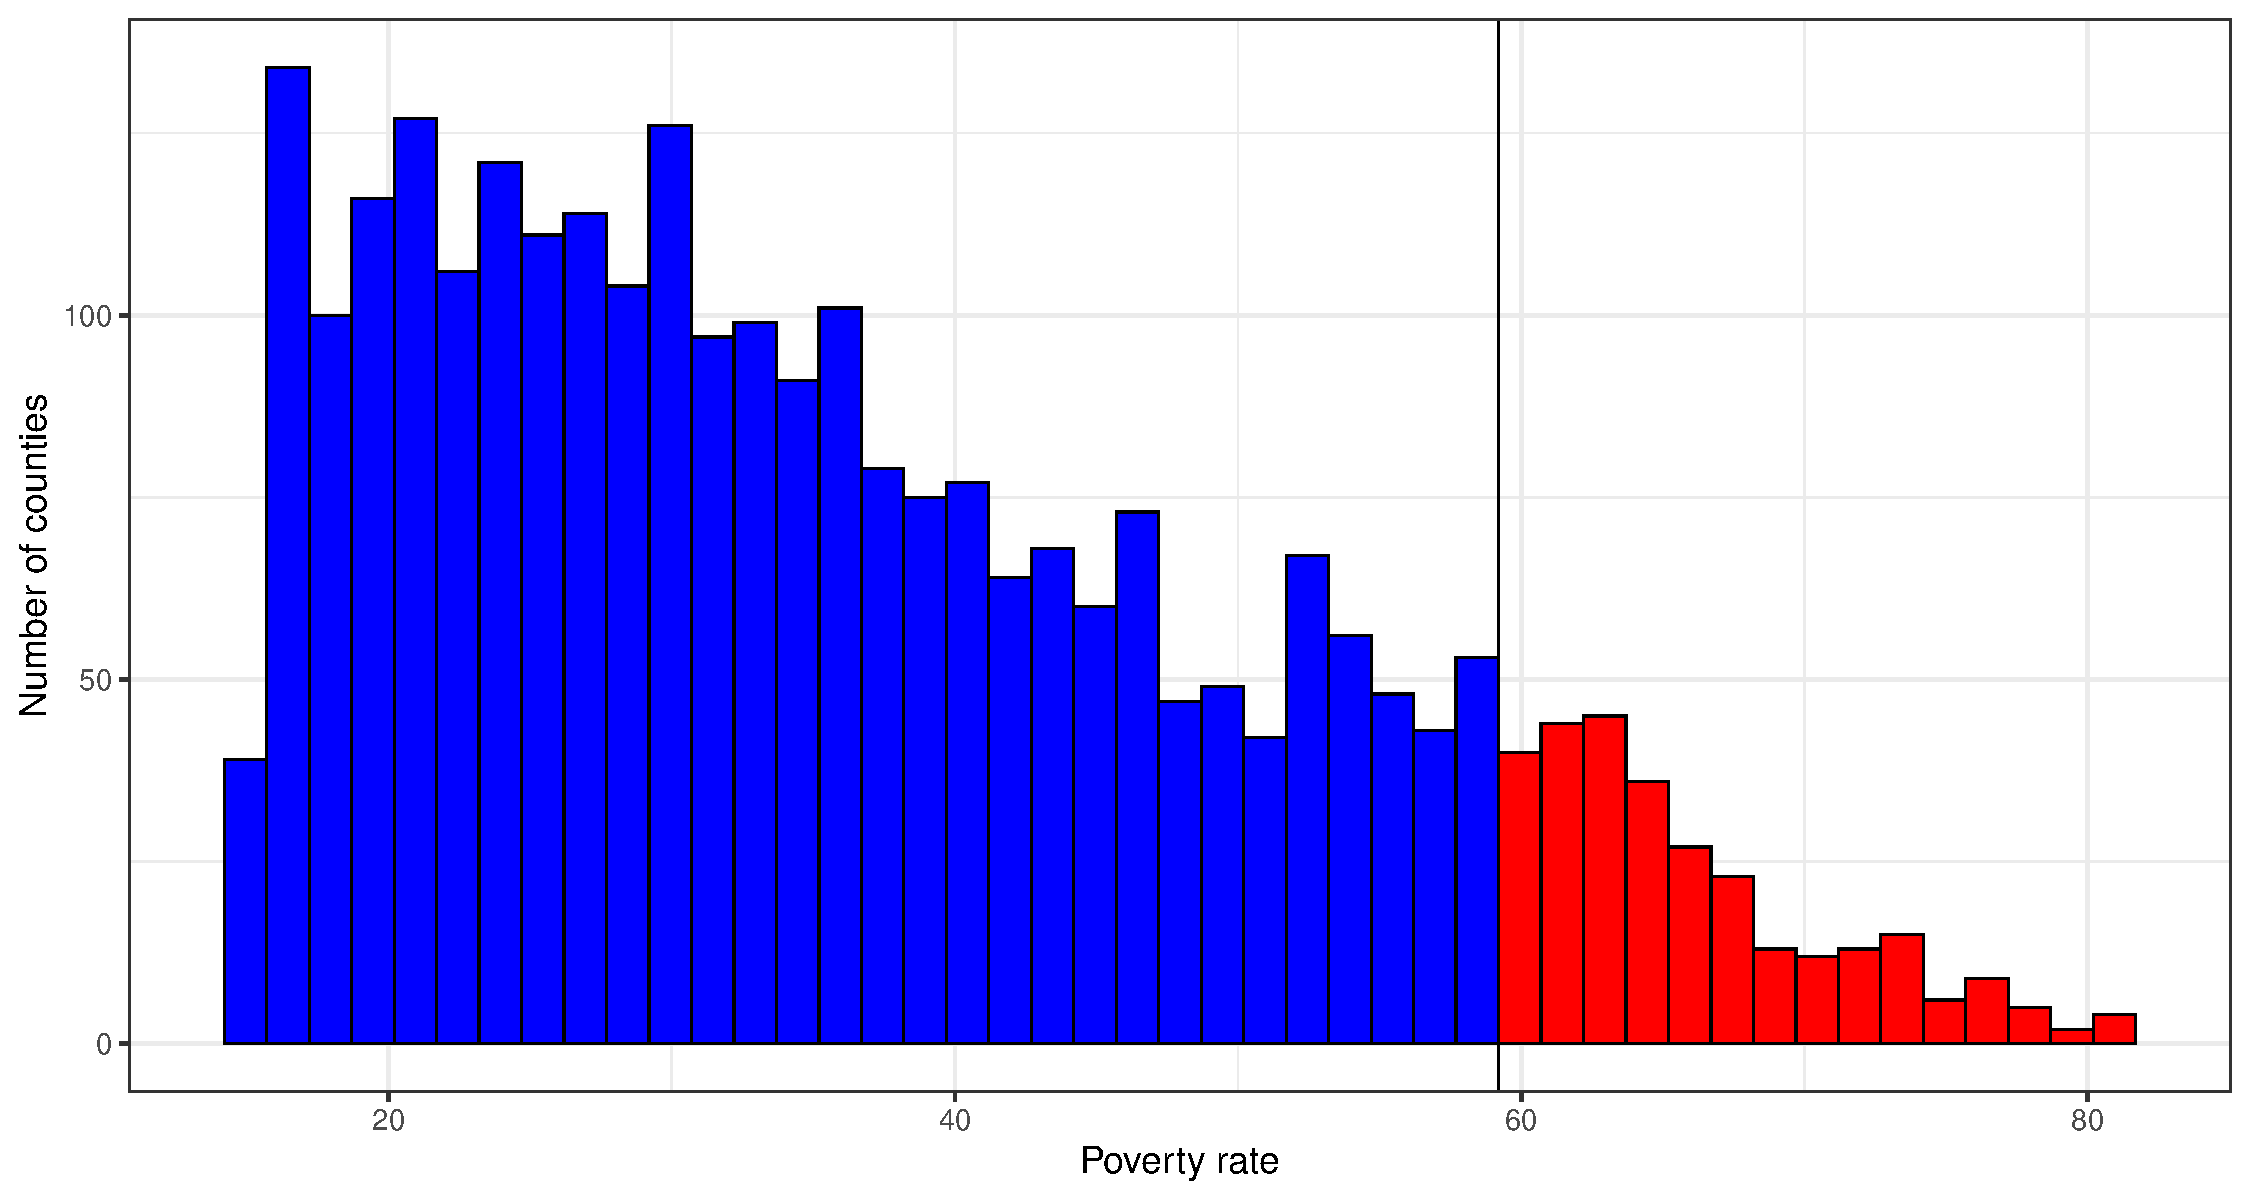
\includegraphics[width=\textwidth]{figure_A04.pdf}
	\caption{Histogram of the poverty rate (assignment variable).
			 The histogram is constructed such that the cutoff (vertical line) constitutes a boundary,
		 	 separating control (blue) and treated (red) counties.}
	\label{fig:histogram}
\end{figure}
\vfill

\clearpage

\vfill
\begin{figure}
	\centering
	\begin{subfigure}[t]{0.49\textwidth}
		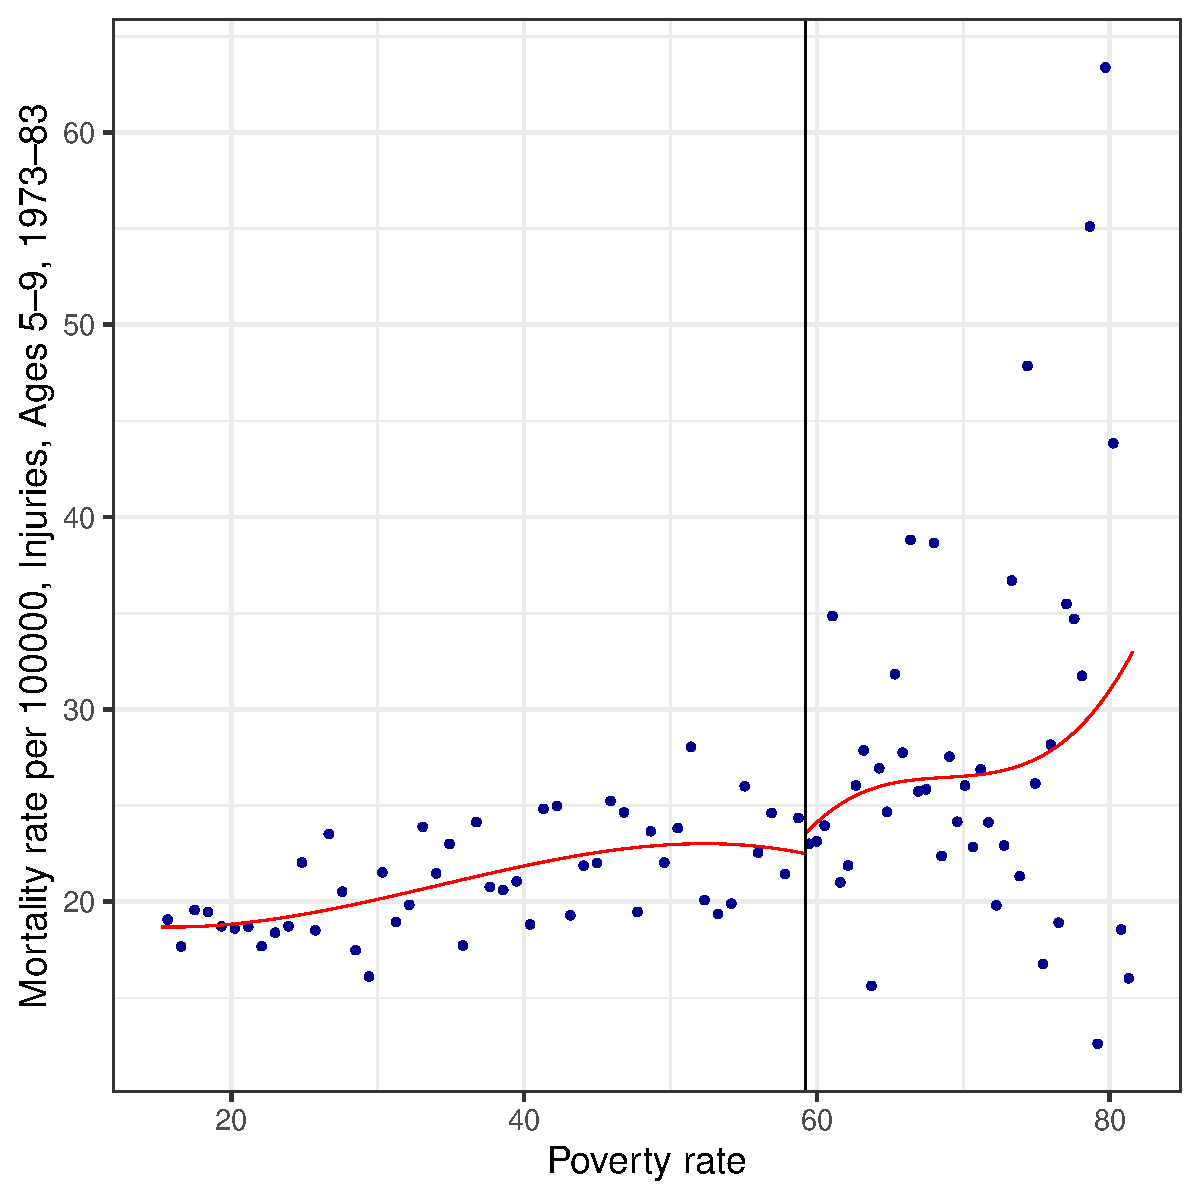
\includegraphics[width=\textwidth]{figure_A05a.pdf}
		\captionsetup{format=hang}
		\caption{Post-treatment placebo outcome injury-related mortality}
		\label{fig:rdplot_injury}
	\end{subfigure}
	\begin{subfigure}[t]{0.49\textwidth}
		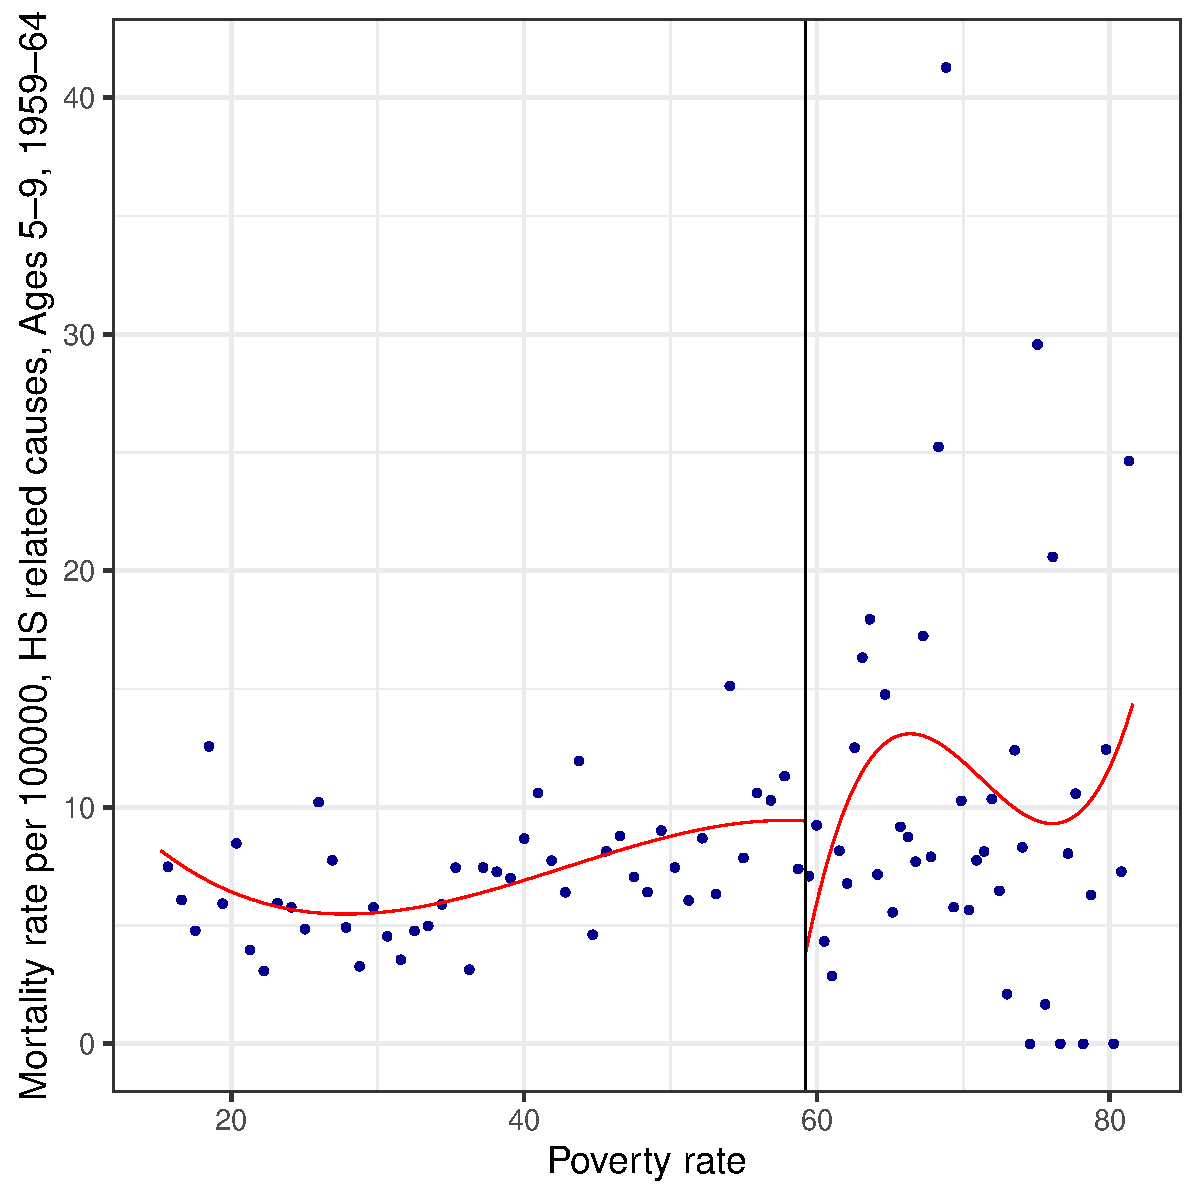
\includegraphics[width=\textwidth]{figure_A05b.pdf}
		\caption{Outcome of interest $(Y)$ before treatment}
		\label{fig:rdplot_Y_pre}
	\end{subfigure}
	\caption{RD plot for two covariates where no treatment effect is expected, to provide evidence for the validity of the RD design.
			 The dots depict the mean within each bin, where the bins are evenly spaced and their number is chosen to mimic variance.
		 	 The solid red lines are third-order polynomial fits for control (left) and treated (right) counties separately.}
	\label{fig:rdplots_cov}
\end{figure}
\vfill
\begin{figure}
	\centering
	\begin{subfigure}[t]{0.49\textwidth}
		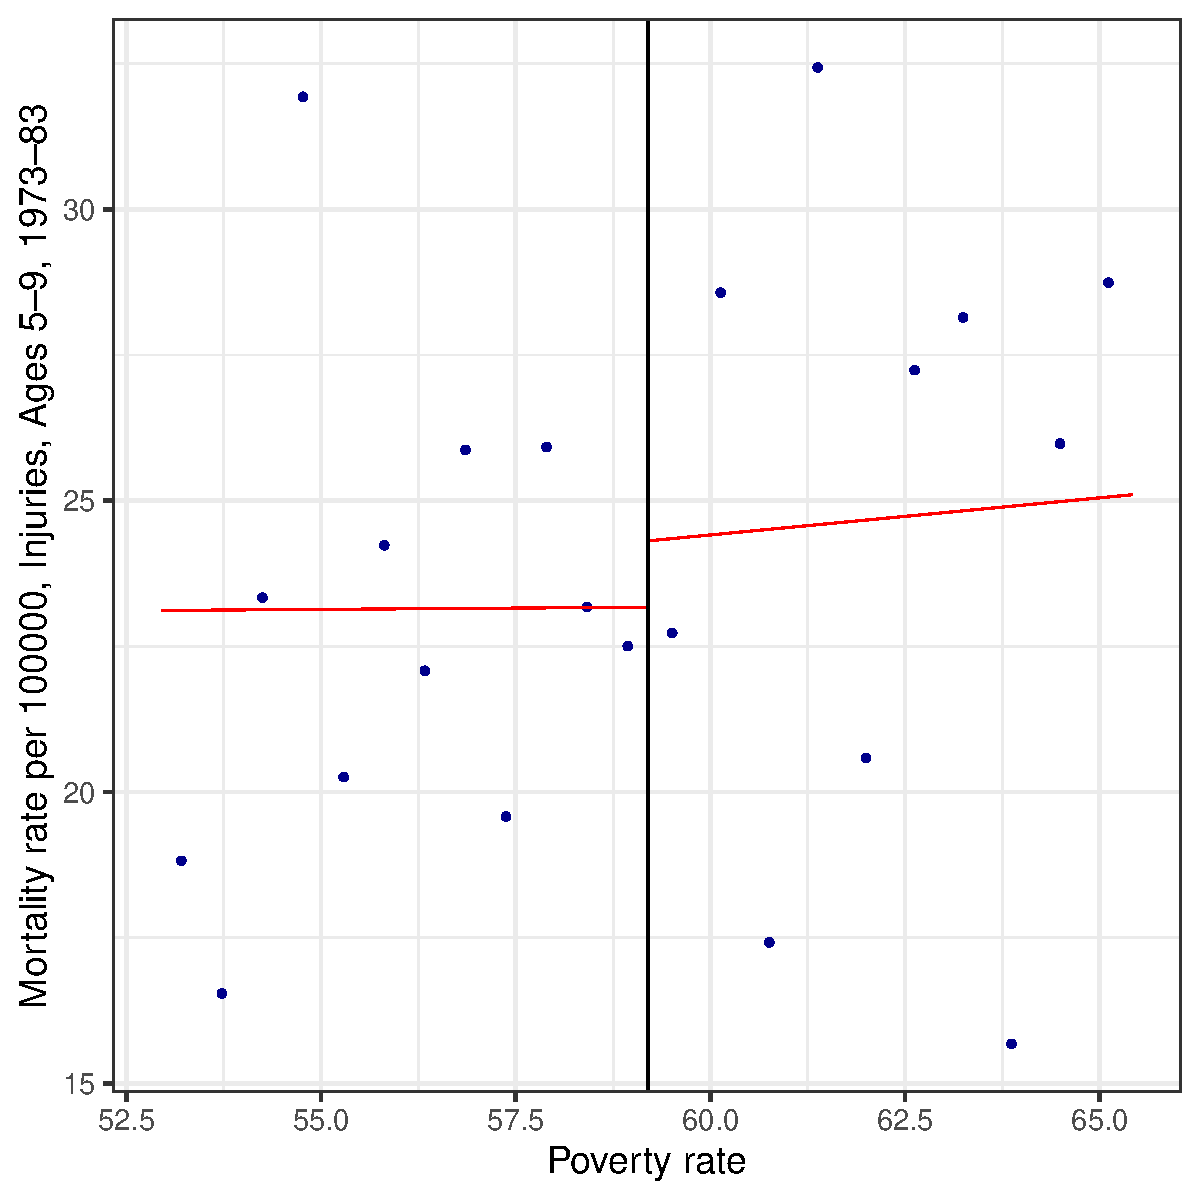
\includegraphics[width=\textwidth]{figure_A06a.pdf}
		\captionsetup{format=hang}
		\caption{Post-treatment placebo outcome injury-related mortality}
		\label{fig:llplot_injury}
	\end{subfigure}
	\begin{subfigure}[t]{0.49\textwidth}
		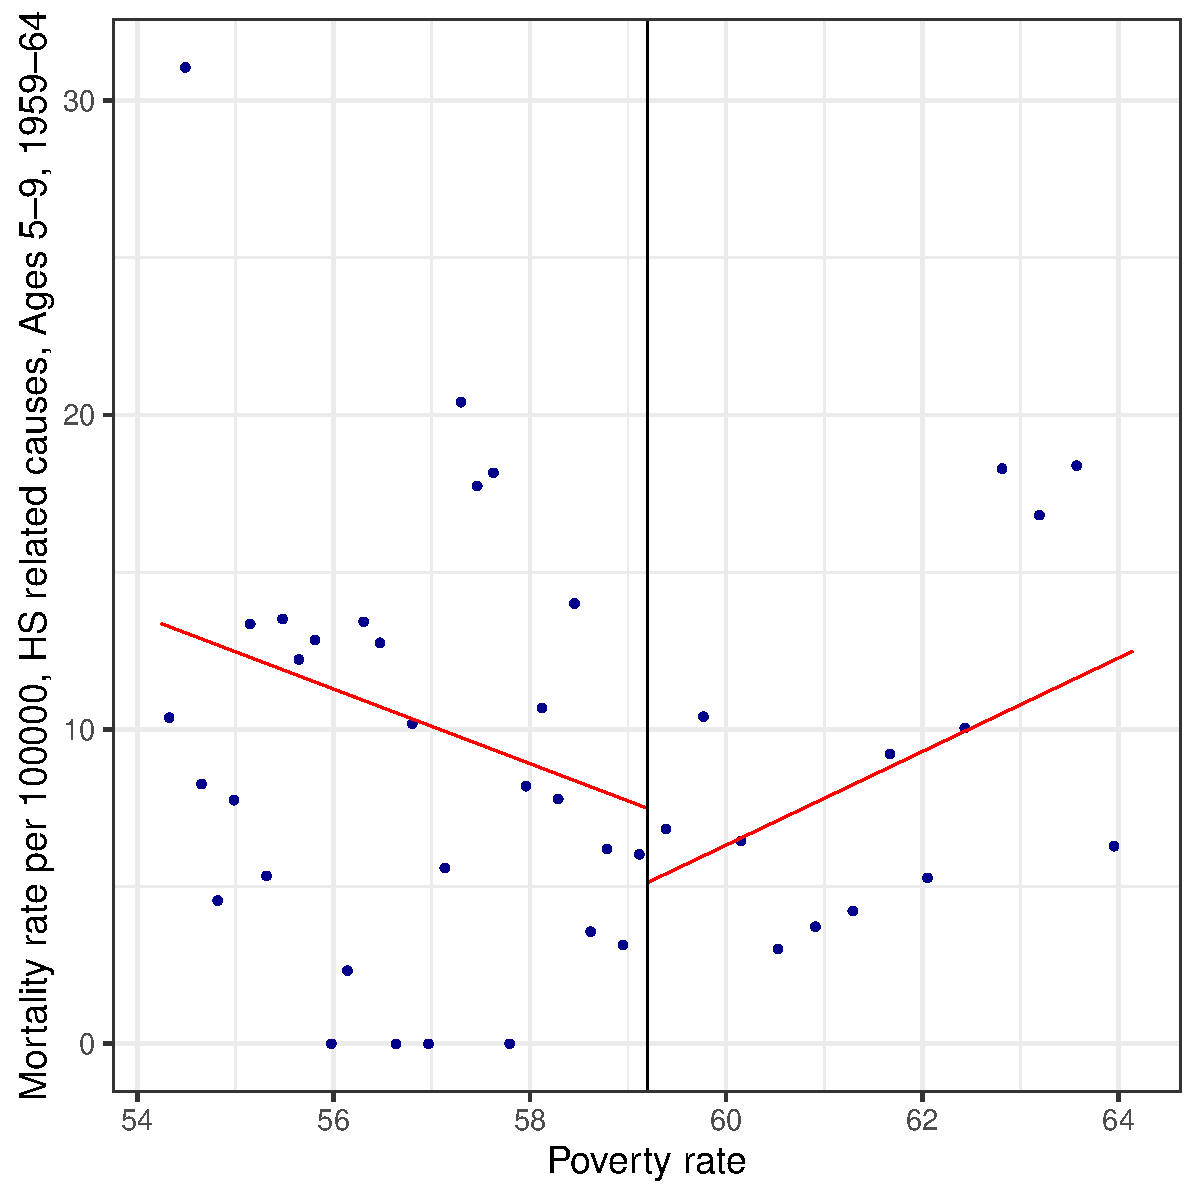
\includegraphics[width=\textwidth]{figure_A06b.pdf}
		\caption{Outcome of interest $(Y)$ before treatment}
		\label{fig:llplot_Y_pre}
	\end{subfigure}
	\caption{As Figure~\ref{fig:rdplots_cov}, but instead of global polynomial fits the local linear fits
			 (triangular kernel, estimated MSE-optimal bandwidth) are displayed.}
	\label{fig:llplots_cov}
\end{figure}
\vfill

\clearpage

\begin{landscape}
\renewcommand{\arraystretch}{1.2}
\begin{table}[p]
	\centering
	\captionabove{RD effect analysis for covariates}
	\label{tab:covariates}
	\begin{tabular}{l r r c c}  
		\toprule
		\multirow{2}[1]{*}{Covariate} & \multirow{2}[1]{*}{$\hat{h}_{\text{MSE}}$} & \multirow{2}[1]{*}{RD estimate} & \multicolumn{2}{c}{RBC inference} \\
		\cmidrule(lr){4-5} 
		& & & 95\% CI & $p$-value \\
		\midrule
		Mortality, Injuries, Ages 5--9, 1973--1983                  & 6.262  & 1.133    & [$-$7.074, 10.120]       & 0.728 \\
		Mortality, All causes, Ages 5--9, 1973--1983                & 6.345  & $-$3.501 & [$-$14.679, 7.371]       & 0.516 \\
		Mortality, Head Start related causes, Ages 25+, 1973--1983  & 8.054  & 2.032    & [$-$12.557, 14.913]      & 0.866 \\
		Mortality, Injuries, Ages 25+, 1973--1983                   & 6.205  & 0.052    & [$-$13.815, 9.693]       & 0.731 \\
		Mortality, Head Start related causes, Ages 5--9, 1959--1964 & 4.963  & $-$2.376 & [$-$7.009, 3.476]        & 0.509 \\
		Census 1960: County population                              & 9.352  & 3084.605 & [$-$5920.470, 11918.011] & 0.510 \\
		Census 1960: \% attending school, Ages 14--17               & 10.083 & 0.557    & [$-$4.335, 5.832]        & 0.773 \\
		Census 1960: \% attending school, Ages 5--34                & 6.194  & 0.906    & [$-$1.345, 3.325]        & 0.406 \\
		Census 1960: \% high school or more, Ages 25+               & 7.651  & 0.621    & [$-$1.490, 2.801]        & 0.549 \\
		Census 1960: Population, Ages 14--17                        & 9.642  & 308.801  & [$-$352.227, 1017.850]   & 0.341 \\
		Census 1960: Population, Ages 5--34                         & 9.703  & 1648.581 & [$-$2977.399, 6400.919]  & 0.474 \\
		Census 1960: Population, Ages 25+                           & 8.312  & 1574.977 & [$-$2894.802, 5741.418]  & 0.518 \\
		Census 1960: \% urban population                            & 8.846  & 2.339    & [$-$5.567, 11.564]       & 0.493 \\
		Census 1960: \% black population                            & 7.166  & 0.793    & [$-$10.237, 11.035]      & 0.941 \\
		\bottomrule \addlinespace[0.25ex]
		\multicolumn{5}{l}{\footnotesize \textit{Note}: Results are based on local linear estimation and the triangular kernel.}
	\end{tabular}	
\end{table}
\renewcommand{\arraystretch}{1.0}
\end{landscape}

\begin{table}[h]
	\centering
	\captionabove{RD effect analysis for placebo cutoffs}
	\label{tab:placebo_cutoffs}
	\begin{tabular}{c c c c c}  
		\toprule
		\multirow{2}[1]{*}{Cutoff} & \multirow{2}[1]{*}{$\hat{h}_{\text{MSE}}$} & \multirow{2}[1]{*}{RD estimate} & \multicolumn{2}{c}{RBC inference} \\
		\cmidrule(lr){4-5} 
		& & & 95\% CI & $p$-value \\
		\midrule
		\multicolumn{5}{c}{Below true cutoff} \\[0.25ex]
		31.463 & 4.595 & \minwd0.032 & [$-$1.142, 1.420]    & 0.831 \\
		40     & 6.114 & \minwd0.015 & [$-$1.494, 2.019]    & 0.769 \\
		50     & 2.340 & \minwd1.894 & [$-$1.689, 6.397]    & 0.254 \\[1ex]
		\multicolumn{5}{c}{True cutoff} \\[0.25ex]
		59.198 & 6.913 & $-$2.389    & [$-$5.426, $-$0.083] & 0.043 \\[1ex]
		\multicolumn{5}{c}{Above true cutoff} \\[0.25ex]
		64.428 & 2.024 & $-$0.490    & [$-$2.802, 2.223]    & 0.821 \\
		70     & 3.054 & $-$1.733    & [$-$15.334, 10.639]  & 0.723 \\
		\bottomrule \addlinespace[0.25ex]
		\multicolumn{5}{l}{\footnotesize \textit{Note}: The median poverty rate for control is 31.463, and for treatment 64.428.} \\[-0.75ex]
		\multicolumn{5}{l}{\footnotesize Results are based on local linear estimation and the triangular kernel.}
	\end{tabular}	
\end{table}

\begin{table}[h]
	\centering
	\captionabove{RD effect analysis for the donut-hole-approach}
	\label{tab:donut_holes}
	\begin{tabular}{c c c c c c c}  
		\toprule
		Radius & \multirow{2}[1]{*}{$\hat{h}_{\text{MSE}}$} & \multirow{2}[1]{*}{RD estimate} & \multicolumn{2}{c}{RBC inference} & \multicolumn{2}{c}{Excluded counties} \\
		\cmidrule(lr){4-5} \cmidrule(lr){6-7} 
		donut hole & & & 95\% CI & $p$-value & Control & Treatment \\
		\midrule
		0.0 & 6.913 & $-$2.389 & [$-$5.426, $-$0.083] & 0.043 & 0  & 0  \\
		0.1 & 6.524 & $-$2.515 & [$-$5.821, $-$0.030] & 0.048 & 3  & 3  \\
		0.2 & 6.371 & $-$2.208 & [$-$5.744, 0.564]    & 0.107 & 6  & 8  \\
		0.3 & 6.407 & $-$1.966 & [$-$5.604, 0.979]    & 0.168 & 9  & 10 \\
		0.4 & 6.438 & $-$2.143 & [$-$6.136, 1.045]    & 0.165 & 12 & 12 \\
		0.5 & 6.468 & $-$2.478 & [$-$7.196, 1.309]    & 0.175 & 18 & 16 \\
		\bottomrule \addlinespace[0.25ex]
		\multicolumn{7}{l}{\footnotesize \textit{Note}: Results are based on local linear estimation and the triangular kernel.}
	\end{tabular}	
\end{table}

\clearpage

\nocite{R_2023} 
\printbibliography

\newpage

\newgeometry{top=2cm, left=2cm, right=2cm, bottom=2cm}

\thispagestyle{empty}
\section*{Statement of authorship}

I hereby confirm that the work presented has been performed and interpreted solely by myself
except for where I explicitly identified the contrary.
I assure that this work has not been presented in any other form for the fulfillment of any other degree or qualification.
Ideas taken from other works in letter and in spirit are identified in every single case.

\vspace{3cm}

\begin{center}
	\parbox{6cm}{\hrule \strut \centering Place, Date} \hspace{1.5cm} \parbox{6cm}{\hrule \strut \centering Signature}	 	
\end{center}

\end{document}